\documentclass[a4paper, 12pt]{book}
\usepackage{amssymb}
\usepackage[italian]{babel}
\usepackage{xspace}
\usepackage{tikz}
\usepackage[newitem,newenum,neverdecrease]{paralist}
\usepackage{amsmath,amssymb,amsfonts,mathrsfs,latexsym,stmaryrd}
\usepackage{mathtools}
\usepackage{amsthm}
\usepackage{ifpdf}
\usepackage{cases}
\usepackage{ragged2e} 	% https://tex.stackexchange.com/questions/89680/how-can-one-set-full-justification-within-left-justified-raggedright-text
\usepackage{breakcites} % https://tex.stackexchange.com/questions/2773/how-do-i-make-latex-push-long-citations-to-a-new-line
\usepackage{hyperref}	% http://tex.stackexchange.com/questions/73862/how-can-i-make-a-clickable-table-of-contents
\usepackage{fancyhdr}	% https://www.sharelatex.com/blog/2013/08/06/thesis-series-pt2.html
\usepackage{titlesec} 	% http://tex.stackexchange.com/questions/11444/how-to-format-the-chapter-heading
\usepackage[T1]{fontenc}
\usepackage[utf8]{inputenc}
\usepackage{xcolor}
\usepackage{geometry}
\usepackage{layout}		% http://tex.stackexchange.com/questions/50258/margins-of-book-class
\usepackage{pseudocode}
\usepackage{chngcntr}


% fixes for pseudocode-hyperref interaction
\counterwithout{pseudocode}{section}
%\counterwithin{pseudocode}{chapter}
\renewcommand{\thepseudocode}{\thechapter.\arabic{pseudocode}}

\newcounter{newpseudonum}[pseudocode]
\renewcommand{\thenewpseudonum}{\thepseudocode\alph{newpseudonum}}
\providecommand{\labelline}[2][0.5in]{&\refstepcounter{newpseudonum}\hspace*{#1}\mbox{(\thenewpseudonum)}\label{#2}}
\ifpdf
  \providecommand{\refline}[1]{\hyperref[#1]{(\ref*{#1})}}
\else
  \providecommand{\refline}[1]{\ref*{#1}}
\fi
\newcommand{\pcodetab}[1]{\hspace*{#1ex}}

% alignement fixes for pseudocode blocks
\renewcommand{\DO}{\\\!\!\pcodetab{1}\mbox{ \bfseries \makebox[0pt][l]{do}\phantom{xx} }}
\renewcommand{\ELSE}{\\\pcodetab{1}\mbox{ \bfseries \makebox[0pt][l]{else}\phantom{then} }}
\renewcommand{\RETURN}[1]{\ifthenelse{\equal{#1}{} }{\mbox{\bfseries return}}{\mbox{\bfseries return}#1}}
\newcommand{\FUNCTION}[2]{\mbox{\bfseries proc }\mbox{\textsc{#1}}\left(\ensuremath{#2}\right)\\}
\newcommand{\ENDFUNCTION}{}
\newcommand{\FCALL}[2]{\mbox{\textsc{#1}}\left(\ensuremath{#2}\right)\\}



% code box length
\newlength{\pcodewidth}
\setlength{\pcodewidth}{\textwidth}
\addtolength{\pcodewidth}{-58pt}

% code environment
\newenvironment{code}[1]{
\begin{Sbox}
\!\!\begin{minipage}{#1}%\pcodewidth}
\bfseries
\noindent
%\begin{math}
\small
$$
\begin{array}{@{\hspace*{1ex}}lr@{}}
}{
\end{array}
$$
%\end{math}
\end{minipage}\vspace{-2mm}
\end{Sbox}
\shadowbox{\TheSbox}{}
}	% For pseudocodes
\usepackage{csquotes}
\usepackage{listings} % Per la visualizzazione del codice
\usepackage{xcolor}
\usepackage{graphicx} % Per l'inserimento di immagini
\usepackage{caption}
\usepackage{float}
\usepackage{longtable} % Per realizzazione tabelle database
\usepackage{ltablex}
\usepackage{multirow}
\usepackage{tabularx}
\usepackage[a-1b]{pdfx} % Per conversione in PDF/A
\usepackage[backend=bibtex, citestyle=numeric, sorting=none]{biblatex}
\addbibresource{bibliografia-tesi-Taiwo-Solomon.bib}

\lstset{
    basicstyle=\ttfamily\small, % Stile di base per il codice (font monospazio)
    breaklines=true,            % Consenti a righe lunghe di andare a capo
    numbers=left,               % Mostra i numeri di riga a sinistra
    numberstyle=\tiny,          % Stile dei numeri di riga
    frame=single,               % Aggiungi una cornice attorno al codice
    captionpos=b,               % Posiziona la didascalia sotto il codice
    showstringspaces=false,     % Non mostrare gli spazi nelle stringhe
}

% Aumentare l'altezza dell'intestazione e compensare il margine superiore
\setlength{\headheight}{15pt}

%%% Formattazione del header del Capitolo
\titleformat
{\chapter} % command
[display] % shape
{\bfseries\Huge\bfseries} % format
{\flushright \color{black!45}{\Large Capitolo \thechapter}} % label
{0.2ex} % sep
{
    \rule{\textwidth}{3pt}
    \centering
} % before-code
[
\rule{\textwidth}{3pt}
] % after-code
%%% end

%%% Formattazione dei hyper riferimenti (hyperref)
% hyperref setup -- http://tex.stackexchange.com/questions/73862/how-can-i-make-a-clickable-table-of-contents
\definecolor{Gold}{rgb}{0.55,0.55,0}
\definecolor{DarkGray}{rgb}{0.3, 0.3, 0.3}
\definecolor{black}{rgb}{0.0, 0.0, 0.0}


\hypersetup{
    unicode=false,          % non-Latin characters in Acrobat’s bookmarks
    pdftoolbar=true,        % show Acrobat’s toolbar?
    pdfmenubar=true,        % show Acrobat’s menu?
    pdffitwindow=false,     % window fit to page when opened
    pdfstartview={FitH},    % fits the width of the page to the window
    pdftitle={Interfaccia web per la gestione dei permessi in una piattaforma E-learning per scuole superiori},    % title
    pdfauthor={Taiwo Solomon Olamide},     % author
    pdfsubject={Interfaccia web per la gestione dei permessi in una piattaforma E-learning per scuole superiori},   % subject of the document
    pdfcreator={Taiwo Solomon Olamide},   % creator of the document
    pdfproducer={Taiwo Solomon Olamide}, % producer of the document
    pdfkeywords={Ruby, Ruby on Rails, Vue.js, Quasar, PostgreSQL}, % list of keywords
    linktocpage=false,		% number hyperref'd =true, false otherwise
    pdfnewwindow=true,      % links in new PDF window
    colorlinks=true,       % false: boxed links; true: colored links
    linkcolor=DarkGray,          % color of internal links (change box color with linkbordercolor)
    citecolor=magenta,        % color of links to bibliography
    filecolor=green,      % color of file links
    urlcolor=Gold           % color of external links
}

% https://tex.stackexchange.com/questions/95488/list-of-figures-and-page-numbering
\makeatletter
\newcommand{\emptypage}[1]{%
  \cleardoublepage
  \begingroup
  \let\ps@plain\ps@empty
  \pagestyle{empty}
  #1
  \cleardoublepage}
\makeatletter

% base line strech (default 1.0) -- interlinea
\renewcommand{\baselinestretch}{1.2}

\begin{document}
%%% Nuova geometria per la pagina del titolo
% visto che la classe del documento è book, le pagine pari e dispari avranno geometrie diverse,
% mentre quella del titolo deve essere unica!
\newgeometry{
  top=2cm,
  bottom=2cm,
  left=2cm,
  right=2cm,
  headsep=25pt,
  headheight=15pt
}

%%% Pagina del titolo
\begin{titlepage}
  \topskip0pt
  \centering
  \vspace*{5mm}
  
\includegraphics[width=0.5\textwidth]{../images/logo-unife-hires.png}\\
  \vspace*{1cm}
  \huge \textbf{\textsc{Università degli Studi di Ferrara}}
  \Large \textsc{Corso di Laurea in Informatica}

  \vspace*{2.5cm}
  \hrule width \hsize \kern 1mm \hrule width \hsize height 2pt
  \vspace*{10mm}
  \Huge \emph{\textnormal{Interfaccia web per la gestione dei permessi in una piattaforma E-learning per scuole superiori}}
  \vspace*{10mm}
  \hrule width \hsize height 2pt
  \vspace*{1mm}
  \hrule width \hsize \kern 1mm

  \vspace*{3.5cm}
  \begin{minipage}{0.45\textwidth}
    \begin{flushleft} \Large
      \emph{Relatore:}\\
      \Large \textbf{Prof. Fabrizio \textsc{Riguzzi}}
      \emph{Secondo relatore:}\\
      \Large \textbf{Dr. Ing. Arnaud \textsc{Nguembang Fadja}}
    \end{flushleft}
  \end{minipage}
  \begin{minipage}{0.5\textwidth}
    \begin{flushright} \Large
      \emph{Laureando:} \\
      \Large \textbf{Solomon Olamide \textsc{Taiwo}}
    \end{flushright}
  \end{minipage}

  \vfill % Push 'Anno accademico' to the buttom
  \Large \textsc{Anno Accademico $2023/2024$}
\end{titlepage}
\restoregeometry

%%% ---- INDICE -----

\titlespacing{\chapter}{0pt}{-20pt}{20pt}

\pagestyle{empty}
\clearpage
\tableofcontents
\thispagestyle{empty}
\addtocontents{toc}{\protect\thispagestyle{empty}}	% http://tex.stackexchange.com/questions/2995/removing-page-number-from-toc 

%%% ---- FINE INDICE -----

%%% ---- CAPITOLO 'INTRODUZIONE' -----

\chapter*{Introduzione}
\addcontentsline{toc}{chapter}{Introduzione}
%%% Fancy header settings, queste impostazioni vanno fatte solo una volta all'inizio del primo capitolo
\pagestyle{fancy}
\fancyhf{}
\renewcommand{\headrulewidth}{2pt}
\fancyhead[EL]{\textbf{\textsf{\nouppercase\thepage}}}
\fancyhead[ER]{\textbf{\textsf{\nouppercase\leftmark}}}
\fancyhead[OR]{\textbf{\textsf{\nouppercase\thepage}}}
\fancyhead[OL]{\textbf{\textsf{\nouppercase {\rightmark}}}}
%%% end

%%% all'inizio di ogni capitolo, questa impostazione rimuove il numero di pagina, provare a commentare per vedere la differenza
\thispagestyle{empty}

%%% ---- CORPO 'INTRODUZIONE' -----

La presente tesi di laurea trae origine dal lavoro svolto in collaborazione con System Afrik Information Technology \cite{syait}: questa realtà di origine ferrarese
rappresenta un autentico faro di innovazione nel panorama delle tecnologie digitali, posizionandosi come un punto di riferimento per lo sviluppo di
progetti tecnologicamente avanzati che, anche attraverso la collaborazione attiva con l'Università degli Studi di Ferrara,
uniscono la realtà accademica a quella imprenditoriale.\\

Il contatto fra questi due mondi ha portato e sta portando alla realizzazione di soluzioni di alta qualità per clienti di tutto il mondo: una di queste
è la piattaforma E-learning, attualmente in corso di sviluppo e su cui ho avuto il piacere di lavorare, pensata per la gestione di istituti scolastici
desiderosi di garantire ai propri studenti, ai loro familiari ed al personale scolastico un servizio moderno, rapido ed affidabile.\\

L'attività principale svolta è l'implementazione di un modulo volto a gestire i permessi degli utenti utilizzatori del suddetto portale e le
annesse logiche di funzionamento, insieme ai controlli che assicurano l'accesso (o il blocco) a specifiche funzionalità della web application.\\

Le conoscenze acquisite nel corso di laurea sono state fondamentali nell'approccio al codebase e nell'apprendimento rapido delle tecnologie
che poi sono state adoperate nel progetto: queste, che meglio verranno descritte nell'apposito capitolo, includono il linguaggio di programmazione Ruby,
il database PostgreSQL ed i framework Ruby on Rails, Quasar e Vue.js, una libreria JavaScript.\\

Questa tesi si occuperà inizialmente di descrivere i requisiti del progetto, per poi illustrarne le suddette tecnologie utilizzate ed infine
enunciare l'argomento principale, ossia l'implementazione della gestione dei permessi utente.

%% ---- FINE CAPITOLO 'INTRODUZIONE' -----

%%% ---- CAPITOLO 'REQUISITI DEL PROGETTO' -----

\chapter{Requisiti del progetto}

%%% all'inizio di ogni capitolo, questa impostazione rimuove il numero di pagina, provare a commentare per vedere la differenza
\thispagestyle{empty}

%%% ---- CORPO 'REQUISITI DEL PROGETTO' -----

Questo capitolo definisce in dettaglio ciò che deve essere implementato nel codebase applicativo, ossia i requisiti del progetto: questi requisiti sono il fondamento su cui
si basa lo sviluppo del sistema di gestione dei permessi degli utenti nell'ambito della piattaforma E-learning di SYSAIT e fanno da punto di riferimento
nello svolgimento del lavoro.\\

Il principale obiettivo del progetto è, per l'appunto, l'implementazione di un'area dedicata alla gestione dei permessi degli utenti: quest'area deve permettere
agli amministratori, ossia allo staff degli istituti scolastici che fanno affidamento alla piattaforma, di definire e gestire i suddetti permessi,
che ogni singolo utente ha individualmente e nell'ambito del profilo in cui lo stesso è inserito.\\

Queste autorizzazioni, costituite da risorse e azioni potenziali su esse che meglio verranno definite nel capitolo relativo al backend, devono
essere gestibili in modo rapido ed intuitivo - il tutto con un'interfaccia chiara e semplice.\\

Prima di iniziare a scrivere codice, è innanzitutto fondamentale avere chiaro come dovrebbe essere la pagina, sia lato desktop che mobile, e
come dovrebbe funzionare, motivo per cui è essenziale avere un mockup a cui fare riferimento. Inoltre, nel rispetto di uno dei principi più
importanti della programmazione, il DRY (Don't Repeat Yourself), è necessario studiare il codice già implementato al fine di poter riutilizzare
componenti già definiti e, conseguentemente, semplificare la realizzazione di nuovi.\\

Di corredo, ma non meno importante, alla realizzazione di questa interfaccia è il controllo delle autorizzazioni degli utenti nelle pagine e nelle
componenti del progetto che fanno uso delle suddette azioni, affinchè non sia possibile visualizzare o interagire con le pagine per le quali non si disponga dell'appropriata
autorizzazione, fornendo all'utente un messaggio informativo inerente.\\

Riassumento, quindi, è possibile definire i requisiti del progetto nel seguente modo:\\

{\Large\textbf{Requisiti funzionali}}

\begin{itemize}
  \item \textbf{Creazione dei componenti che visualizzano le risorse e le azioni}: attraverso il riutilizzo e l'adattamento di codice già esistente, si andranno a
        creare i componenti necessari a visualizzare le risorse e le azioni che costituiscono i permessi del sito;
  \item  \textbf{Realizzazione del layout della pagina principale}: mediante i componenti realizzati, occorrerà creare l'interfaccia e renderla responsiva,
        visivamente appagante e facile da utilizzare;
  \item \textbf{Gestione dei permessi}: gli amministratori devono poter assegnare agli utenti o ai loro rispettivi profili determinati privilegi
        e accessi alle funzionalità della piattaforma, oppure rimuoverli;
  \item \textbf{Accesso alle funzionalità}: gli utenti, a cui sono stati garantiti o revocati specifici permessi, devono poter agire di conseguenza
        all'interno del portale: devono, cioè, poter visionare ed eseguire le azioni delle quali hanno il rispettivo permesso oppure, in caso negativo,
        visualizzare un messaggio che avvisa del diniego.
\end{itemize}

{\Large\textbf{Requisiti non funzionali}}

\smallskip

Oltre ai requisiti funzionali, il progetto deve soddisfare anche requisiti non funzionali che riguardano prestazioni, sicurezza, usabilità e
manutenibilità del sistema. Questi requisiti, come specificato prima, sono cruciali per garantire un'esperienza utente ottimale e la robustezza
del sistema nel lungo periodo.\\

\textbf{Descrizione del caso d'uso}

Il caso d'uso della gestione dei permessi copre una serie di operazioni che possono essere eseguite
da due categorie di attori, i membri dello staff scolastico e gli amministratori della piattaforma, per amministrare i
permessi degli utenti. Queste operazioni includono l'assegnazione di nuovi permessi,
la modifica dei permessi esistenti, la revoca di permessi e la semplice visualizzazione
dei permessi di un utente.\\

\begin{enumerate}
  \item \textbf{Visualizzazione dei permessi di un utente (o profilo)}: il processo di visualizzazione dei permessi di un
        utente inizia con l'autenticazione dello stesso che, una volta inserite le proprie credenziali, può accedere al
        modulo di gestione dei permessi aprendo - attraverso il menu laterale - la homepage della struttura di riferimento da
        cui, tra le varie azioni, è possibile visionare l'elenco dei membri dello staff dello specifico istituto. A questo
        punto, l'amministratore può selezionare l'utente di cui si desidera visionare i permessi e accedere alla
        relativa pagina;
  \item \textbf{Assegnazione di permessi ad un utente (o profilo)}: quest'azione si svolge in modo molto
        simile alla normale visualizzazione, con la sola differenza che l'utente, per assegnare nuovi permessi, deve selezionare
        il permesso desiderato e decidere di salvare, attraverso l'apposito pulsante di salvataggio, tale assegnazione. Dopo
        l'avvenuto salvataggio, la relativa icona verrà disabilitata e l'amministratore può decidere se fare ulteriori modifiche o meno;
  \item \textbf{Revoca dei permessi di un utente (o profilo)}: la revoca dei permessi di un utente è essenziale per mantenere la
        sicurezza del sistema e segue un processo molto simile a quello dell'assegnazione, con l'unica differenza
        che il checkbox relativo all'azione selezionata sarà, al termine del processo, vuoto.
\end{enumerate}

\textbf{Diagramma del caso d'uso}:

Per rappresentare graficamente questi casi d'uso, è possibile utilizzare un diagrama UML (\texttt{Unified Modeling Language}):

\begin{figure}[H]
  \centering
  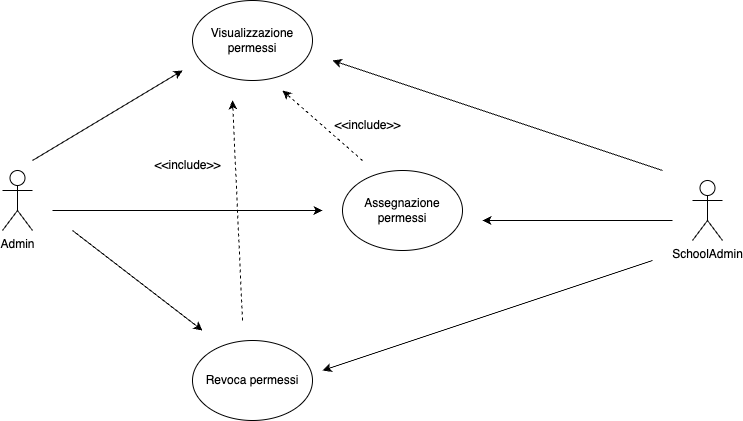
\includegraphics[width=\textwidth]{../images/diagramma-casi-uso-attori.png}
  \caption{Diagramma di caso d'uso per la gestione dei permessi.}
\end{figure}

%% ---- FINE CAPITOLO 'REQUISITI DEL PROGETTO' -----

%%% ---- CAPITOLO 'TECNOLOGIE UTILIZZATE' -----

\chapter{Tecnologie utilizzate}

%%% all'inizio di ogni capitolo, questa impostazione rimuove il numero di pagina, provare a commentare per vedere la differenza
\thispagestyle{empty}

%%% ---- CORPO 'TECNOLOGIE UTILIZZATE' -----

L'implementazione delle pagine e funzionalità descritte nel capitolo precedente richiede l'adozione di una serie di tecnologie avanzate, scelte per la
loro affidabilità, scalabilità e capacità di facilitare lo sviluppo rapido di applicazioni web complesse. Questo capitolo descrive in dettaglio
le principali tecnologie utilizzate nel progetto: Ruby e Ruby on Rails, PostgreSQL, Vue.js e Quasar.\\

Ruby e il suo framework Ruby on Rails sono stati utilizzati per lo sviluppo del backend dell'applicazione, offrendo un ambiente di sviluppo
ricco di funzionalità che permette una rapida iterazione durante il processo di sviluppo.\\

PostgreSQL è stato scelto come sistema di gestione del database per la sua robustezza, per le sue prestazioni e per
la capacità di gestire dati in modo efficiente.\\

Per il frontend, sono stati usati Vue.js e Quasar: Vue.js è una libreria JavaScript progressiva che consente la costruzione di interfacce utente interattive
e dinamiche, mentre Quasar è un framework - basato su Vue.js - che facilita lo sviluppo di interfacce utente moderne e reattive, ottimizzate sia su desktop
che su dispositivi mobili.\\

Nelle sezioni che seguono verranno approfondite queste tecnologie, illustrandone le caratteristiche principali.\\

\section{Ruby e Ruby on Rails}

 {\Large\textbf{Ruby}}\\

Ruby \cite{Ruby} è un linguaggio di programmazione dinamico e orientato agli oggetti, noto per la sua sintassi semplice ed elegante, che enfatizza la produttività del
programmatore e la leggibilità del codice.
Creato da Yuhikiro "Matz" Matsumoto, Ruby combina parti di Perl, Smalltalk, Eiffel, Ada e Lisp.\\

\textbf{Caratteristiche principali}:

\begin{itemize}
  \item \textbf{Sintassi leggibile e concisa}: la sintassi di Ruby è progettata per essere naturale da leggere e facile da scrivere. Ad esempio, un semplice
        programma per stampare "Hello, World!" è scitto come segue:\\
        \begin{lstlisting}[language=ruby]
          puts 'Hello, World!'
        \end{lstlisting}
  \item \textbf{Orientato agli oggetti}: tutto in Ruby è un oggetto, inclusi i tipi di dati primitivi. Ad esempio:\\
        \begin{lstlisting}[language=ruby]
          5.times do
            puts "Hello, World!"
          end
        \end{lstlisting}
        Qui, "5" è un oggetto che ha un metodo "times". Il codice illustrato stampa dunque la stringa "Hello, World!" cinque volte.
  \item \textbf{Dinamicamente tipizzato}: Ruby utilzza un sistema di tipi dinamico e una gestione automatica della memoria. Non è
        necessario dichiarare i tipi delle variabili.
  \item \textbf{Garbage Collection}: Ruby automatizza la gestione della memoria tramite garbage collection, liberando la memoria non più utilizzata.\\
\end{itemize}

{\Large\textbf{Ruby on Rails}}\\

Ruby on Rails \cite{Rails}, spesso semplicemente chiamato Rails, è un framework di sviluppo web open-source basato su Ruby. Creato da David Heinemeier Hansson, Rails
è progettato per facilitare lo sviluppo di applicazioni web seguendo il pradigma Model-View-Controller (MVC).\\

\textbf{Caratteristiche principali}:

\begin{itemize}
  \item \textbf{Convention over Configuration (CoC)}: Rails preferisce le convenzioni rispetto alla configurazione, riducendo la quantità di codice che i
        programmatori devono scrivere.\\
        Ad esempio, seguendo le convenzioni di Rails, la creazione di una risorsa "Article" associa automaticamente le rotte (che sono le definizioni che mappano le URL alle azioni
        corrispondenti nei controller), il controller e le viste necessarie.\\
        \begin{lstlisting}[language=ruby]
          rails generate scaffold Article title:string body:text
        \end{lstlisting}
        Questo comando genera tutto il codice boilerplate per gestire articoli.
  \item \textbf{Don't Repeat Yourself (DRY)}: Rails incoraggia a riutilizzare il codice e a evitare le duplicazioni.
        I moduli e le librerie possono essere inclusi facilmente nei vari componenti dell'applicazione.
  \item \textbf{RESTful design:} Rails promuove l'uso di risorse RESTFUL - che sono un modello di progettazione per le applicazioni web in cui le risorse, rappresentate da URL,
        vengono gestite tramite un insieme standard di operazioni HTTP (GET, POST, PUT, DELETE) che corrispondono alle azioni CRUD (Create, Read, Update, Delete) - per
        sfruttare le applicazioni web, facilitando la creazione di \texttt{API (Application Programming Interface)} ben strutturate e relativamente semplici da gestire.
  \item \textbf{Generazione automatica di codice}: Rails fornisce generatori di codice per lo scaffolding, tecnica che genera automaticamente il codice di base per le
        operazioni CRUD, controller, modelli e altro ancora, accelerando il processo di sviluppo.\\
\end{itemize}

\section{PostgreSQL}

PostgreSQL \cite{PostgreSQL} è un sistema di gestione di database relazionali ad oggetti open-source, noto per la sua robustezza, performance e conformità agli standard SQL. È stato
scelto per la sua capacità di gestire query complesse e volumi di dati elevati, nonchè per le sue caratteristiche avanzate.\\

\textbf{Caratteristiche principali}:

\begin{itemize}
  \item \textbf{ACID Compliance}: PostgreSQL garantisce Atomicità, Consistenza, Isolamento e Durabilità delle transazioni.
        Questo significa che ogni transazione è completamente eseguita oppure completamente annullata.
  \item \textbf{Supporto avanzato per tipi di dati}: include tipi di dati avanzati come JSON e XML. Ad esempio:\\
        \begin{lstlisting}[language=sql]
          CREATE TABLE documents (
          id SERIAL PRIMARY KEY,
          data JSONB
          );
        \end{lstlisting}
        Qui, la colonna 'data' può memorizzare documenti JSON.
  \item \textbf{Estendibilità}: PostreSQL permette l'uso di estensioni per aggiungere funzionalità. Un esempio può essere l'estensione
        PostGIS aggiunge il supporto per dati geografici:\\
        \begin{lstlisting}[language=sql]
          CREATE EXTENSION postgis;
        \end{lstlisting}
  \item \textbf{MVCC (Multi-Version Concurrency Control)}: permette la gestione concorrente delle transazioni senza lock pesanti, migliorando le
        performance in ambienti ad alta concorrenza.\\
  \item \textbf{Backup e ripristino}: offre strumenti robusti per il backup e il ripristino dei dati. Ad esempio, "pg\_dump" è
        utilizzato per creare backup:\\
        \begin{lstlisting}[language=sql]
          pg_dump mydb > db_backup.sql
        \end{lstlisting}
\end{itemize}

\section{Vue.js e Quasar}

 {\Large\textbf{Vue.js}}\\

Vue.js \cite{Vue.js} è una libreria JavaScript progressiva per la costruzione di interfacce utente interattive, creato da Evan You e progettata
per essere incrementale, permettendo ai programmatori di adottare il framework gradualmente.\\

\textbf{Caratteristiche principali}:

\begin{itemize}
  \item \textbf{Componenti reattivi}: Vue.js utilizza componenti reattivi, ossia che rispondono automaticamente ai cambiamenti
        dei dati, aggiornando il DOM in modo efficiente e dinamico per riflettere lo stato attuale dell'applicazione, e modulari
        per costruire interfacce utente. Ad esempio:
        \begin{lstlisting}
        <template>
          <div>
            <p>{{ message }}</p>
            <button @click="reverseMessage">Reverse Message</button>
          </div>
        </template>

        <script>
        export default {
          data() {
            return {
              message: 'Hello, Vue!'
            }
          },
          methods: {
            reverseMessage() {
              this.message = this.message.split('').reverse().join('')
            }
          }
        }
        </script>
      \end{lstlisting}
        Questo codice definisce un componente che visualizza un messaggio e include un pulsante che, quando
        cliccato, inverte il testo del messaggio.
  \item \textbf{Data binding}: offre un binding bidirezionale dei dati per sincronizzare il modello e la vista.
  \item \textbf{Virtual DOM}: usa un DOM virtuale per migliorare le performance delle applicazioni. Il virtual DOM consente di fare aggiornamenti
        efficienti al DOM reale solo quando necessario.
  \item \textbf{Ecosistema ricco}: include strumenti come Vue Router per il routing e Vuex per la gestione dello stato. Ad esempio, Vue Router
        permette di definire le rotte dell'applicazione:\\
        \begin{lstlisting}
          import Vue from 'vue'
          import Router from 'vue-router'
          import Home from '@/components/Home'

          Vue.use(Router)

          export default new Router({
            routes: [
              {
                path: '/',
                name: 'Home',
                component: Home
              }
            ]
          })
        \end{lstlisting}
  \item \textbf{Facilità di integrazione}: può essere integrato facilmente in progetti esistenti senza sovrascrivere il codice.\\
\end{itemize}

\newpage

{\Large\textbf{Quasar}}\\

Quasar \cite{Quasar} è un framework basato su Vue.js che facilita lo sviluppo di applicazioni web responsive, ossia capaci di adattarsi
ed essere fruibili su un'alta gamma di dispositivi, e interattive. Consente di creare applicazioni
multipiattaforma con un unico codice base.\\

\textbf{Caratteristiche principali}:

\begin{itemize}
  \item \textbf{Componenti UI predefiniti}: include una vasta gamma di componenti UI pronti all'uso. Ad esempio:\\
        \begin{lstlisting}
        <template>
          <q-btn label="Click me" @click="handleClick" />
        </template>

        <script>
        export default {
          methods: {
            handleClick() {
              this.$q.notify({
                message: 'Bottone premuto!',
                color: 'green'
              })
            }
          }
        }
        </script>
        \end{lstlisting}
        Questo codice Vue.js utilizza il framework Quasar per creare un semplice pulsante che, quando cliccato,
        mostra una notifica. Nel template, viene definito un pulsante <q-btn> con l'etichetta "Click me" e un
        evento @click che chiama il metodo handleClick quando il pulsante viene premuto. Nella parte script,
        il componente esporta un oggetto che include un metodo handleClick. Questo metodo utilizza \$q.notify
        per visualizzare una notifica con il messaggio "Bottone premuto!" di colore verde.
  \item \textbf{Sviluppo multipiattaforma}: supporta la creazione di applicazioni web, mobile (iOS e Android) e desktop (con Electron).
  \item \textbf{Prestazioni ottimizzate}: include strumenti per ottimizzare le prestazioni e ridurre il tempo di caricamento, come il
        lazy loading dei componenti.
  \item \textbf{CLI potente}: Quasar CLI (\texttt{Command Line Interface}, ossia 'Interfaccia a riga di comando',
        che consente agli utenti di interagire con il software tramite comandi testuali inseriti in una console o terminale)
        facilita la gestione e la configurazione del progetto, permettendo
        di generare rapidamente scaffolding per nuove applicazioni.\\
        \begin{lstlisting}
          quasar create my-project
        \end{lstlisting}
  \item \textbf{Supporto per PWA}: permette di sviluppare Progressive Web Apps, ossia applicazioni web che utilizzano le più
        recenti tecnologie web per offrire un'esperienza utente simile a quella delle applicazioni native, inclusa
        l'accessibilità offline, le notifiche push e l'installazione sul dispositivo con facilità.\\
\end{itemize}

{\Large\textbf{Altre tecnologie}}\\

\textbf{Sistema di versionamento (Git)}

Il controllo versione del codice svolge un ruolo cruciale nello sviluppo software moderno, consentendo ai team di lavorare in
modo collaborativo, tenere traccia delle modifiche e gestire il codice in modo efficiente.\\

Nel progetto è stato adottato Git \cite{Git} come sistema di versionamento principale, che fornisce un modo flessibile e affidabile per gestire
il codice, consentendo di lavorare in branch separati, collaborare su funzionalità diverse contemporaneamente e integrare facilmente
le modifiche tramite pull requests.\\

Di seguito i comandi più utilizzati:\\

{\small\textbf{Inizializzazione di un repository}}
\begin{lstlisting}[language=bash]
    git init
  \end{lstlisting}

{\small\textbf{Aggiunta di un file al repository}}
\begin{lstlisting}[language=bash]
    git add <file>
  \end{lstlisting}

{\small\textbf{Creazione di un commit}}
\begin{lstlisting}[language=bash]
    git commit -m "Messaggio del commit"
  \end{lstlisting}

{\small\textbf{Caricamento del commit al repository remoto}}
\begin{lstlisting}[language=bash]
    git push
  \end{lstlisting}

{\small\textbf{Aggiornamento della repository locale}}
\begin{lstlisting}[language=bash]
    git pull
  \end{lstlisting}

{\small\textbf{Creazione di una nuova branch}}
\begin{lstlisting}[language=bash]
    git checkout -b <nome_branch>
  \end{lstlisting}

{\small\textbf{Merging di una nuova branch}}
\begin{lstlisting}[language=bash]
  git merge <nome_branch>
  \end{lstlisting}

{\small\textbf{Visualizzazione dello stato}}
\begin{lstlisting}[language=bash]
    git status
  \end{lstlisting}

{\small\textbf{Visualizzazione dei log}}
\begin{lstlisting}[language=bash]
  git log
  \end{lstlisting}

\textbf{Hosting delle repositories (Bitbucket)}

Per ospitare le repositories Git e facilitare la collaborazione tra i membri del team, è stato utilizzato Bitbucket, strumento che fornisce
un'infrastruttura sicura e scalabile per archiviare il codice, con funzionalità avanzate come il controllo degli accessi basato su ruoli, il
tracciamento delle issue e la gestione delle pull request.\\

\textbf{Documentazione del progetto (Confluence)}

Per gestire la documentazione del progetto è stata usata Confluence \cite{Confluence}, piattaforma di gestione delle conoscenze e della collaborazione, che fornisce
uno spazio centralizzato per creare, organizzare e condividere documentazione importante, come specifiche dei requisiti, documenti tecnici,
guide per gli sviluppatori e altro ancora.

%% ---- FINE CAPITOLO 'TECNOLOGIE UTILIZZATE' -----

%%% ---- CAPITOLO 'IMPLEMENTAZIONE DELLA GESTIONE DEI PERMESSI' -----

\chapter{Implementazione della gestione dei permessi utente}

%%% all'inizio di ogni capitolo, questa impostazione rimuove il numero di pagina, provare a commentare per vedere la differenza
\thispagestyle{empty}

%%% ---- CORPO 'FRONTEND' -----

\section{Gestione del frontend dei permessi}

Nell'era digitale moderna, il web design ha assunto un ruolo cruciale nel determinare il successo di una piattaforma: un
design efficace e semplice da usare non solo migliora l'esperienza dell'utente, ma aumenta anche l'efficienza operativa
e la soddisfazione complessiva. Esso deve inoltre essere intuitivo, accessibile e reattivo, garantendo che gli utenti
possano navigare e utilizzare le funzionalità della piattaforma senza incontrare ostacoli.\\

Una delle principali sfide nel design delle interfacce utente (UI) è trovare l'equilibrio tra funzionalità e
usabilità, infatti esse dovrebbero offrire tutte le funzionalità necessarie senza risultare complesse o sovraccariche.\\

Questo principio è particolarmente rilevante nel contesto della piattaforma e-learning, dove sia le funzionalità che
i dispositivi utilizzati variano enormemente e occorre trovare un equilibrio per soddisfare la più ampia
platea possibile, senza sovraccaricare l'utente e l'interfaccia.\\

Dal punto di vista tecnico, un web design efficace segue le best practice del responsive design, garantendo che
l'interfaccia sia ottimizzata per vari dispositivi, dai desktop ai dispositivi mobili.

\subsection{Design adottato}

L'interfaccia utente per la gestione dei permessi, inizialmente progettata sotto forma di mockup
da usare come riferimento durante l'implementazione (mostrata nelle figure 3.1 e 3.2), è intuitiva e facile da usare,
sia per dispositivi desktop che mobili.\\

Nella versione desktop, l'interfaccia utente è organizzata in modo chiaro e funzionale: in cima
alla pagina è presente un'intestazione con il titolo "Permission Management", sotto la quale vengono
visualizzate le informazioni dell'utente, tra cui il nome completo, il numero di contatto, l'indirizzo email e il
profilo a cui appartiene.\\

\begin{figure}[H]
  \centering
  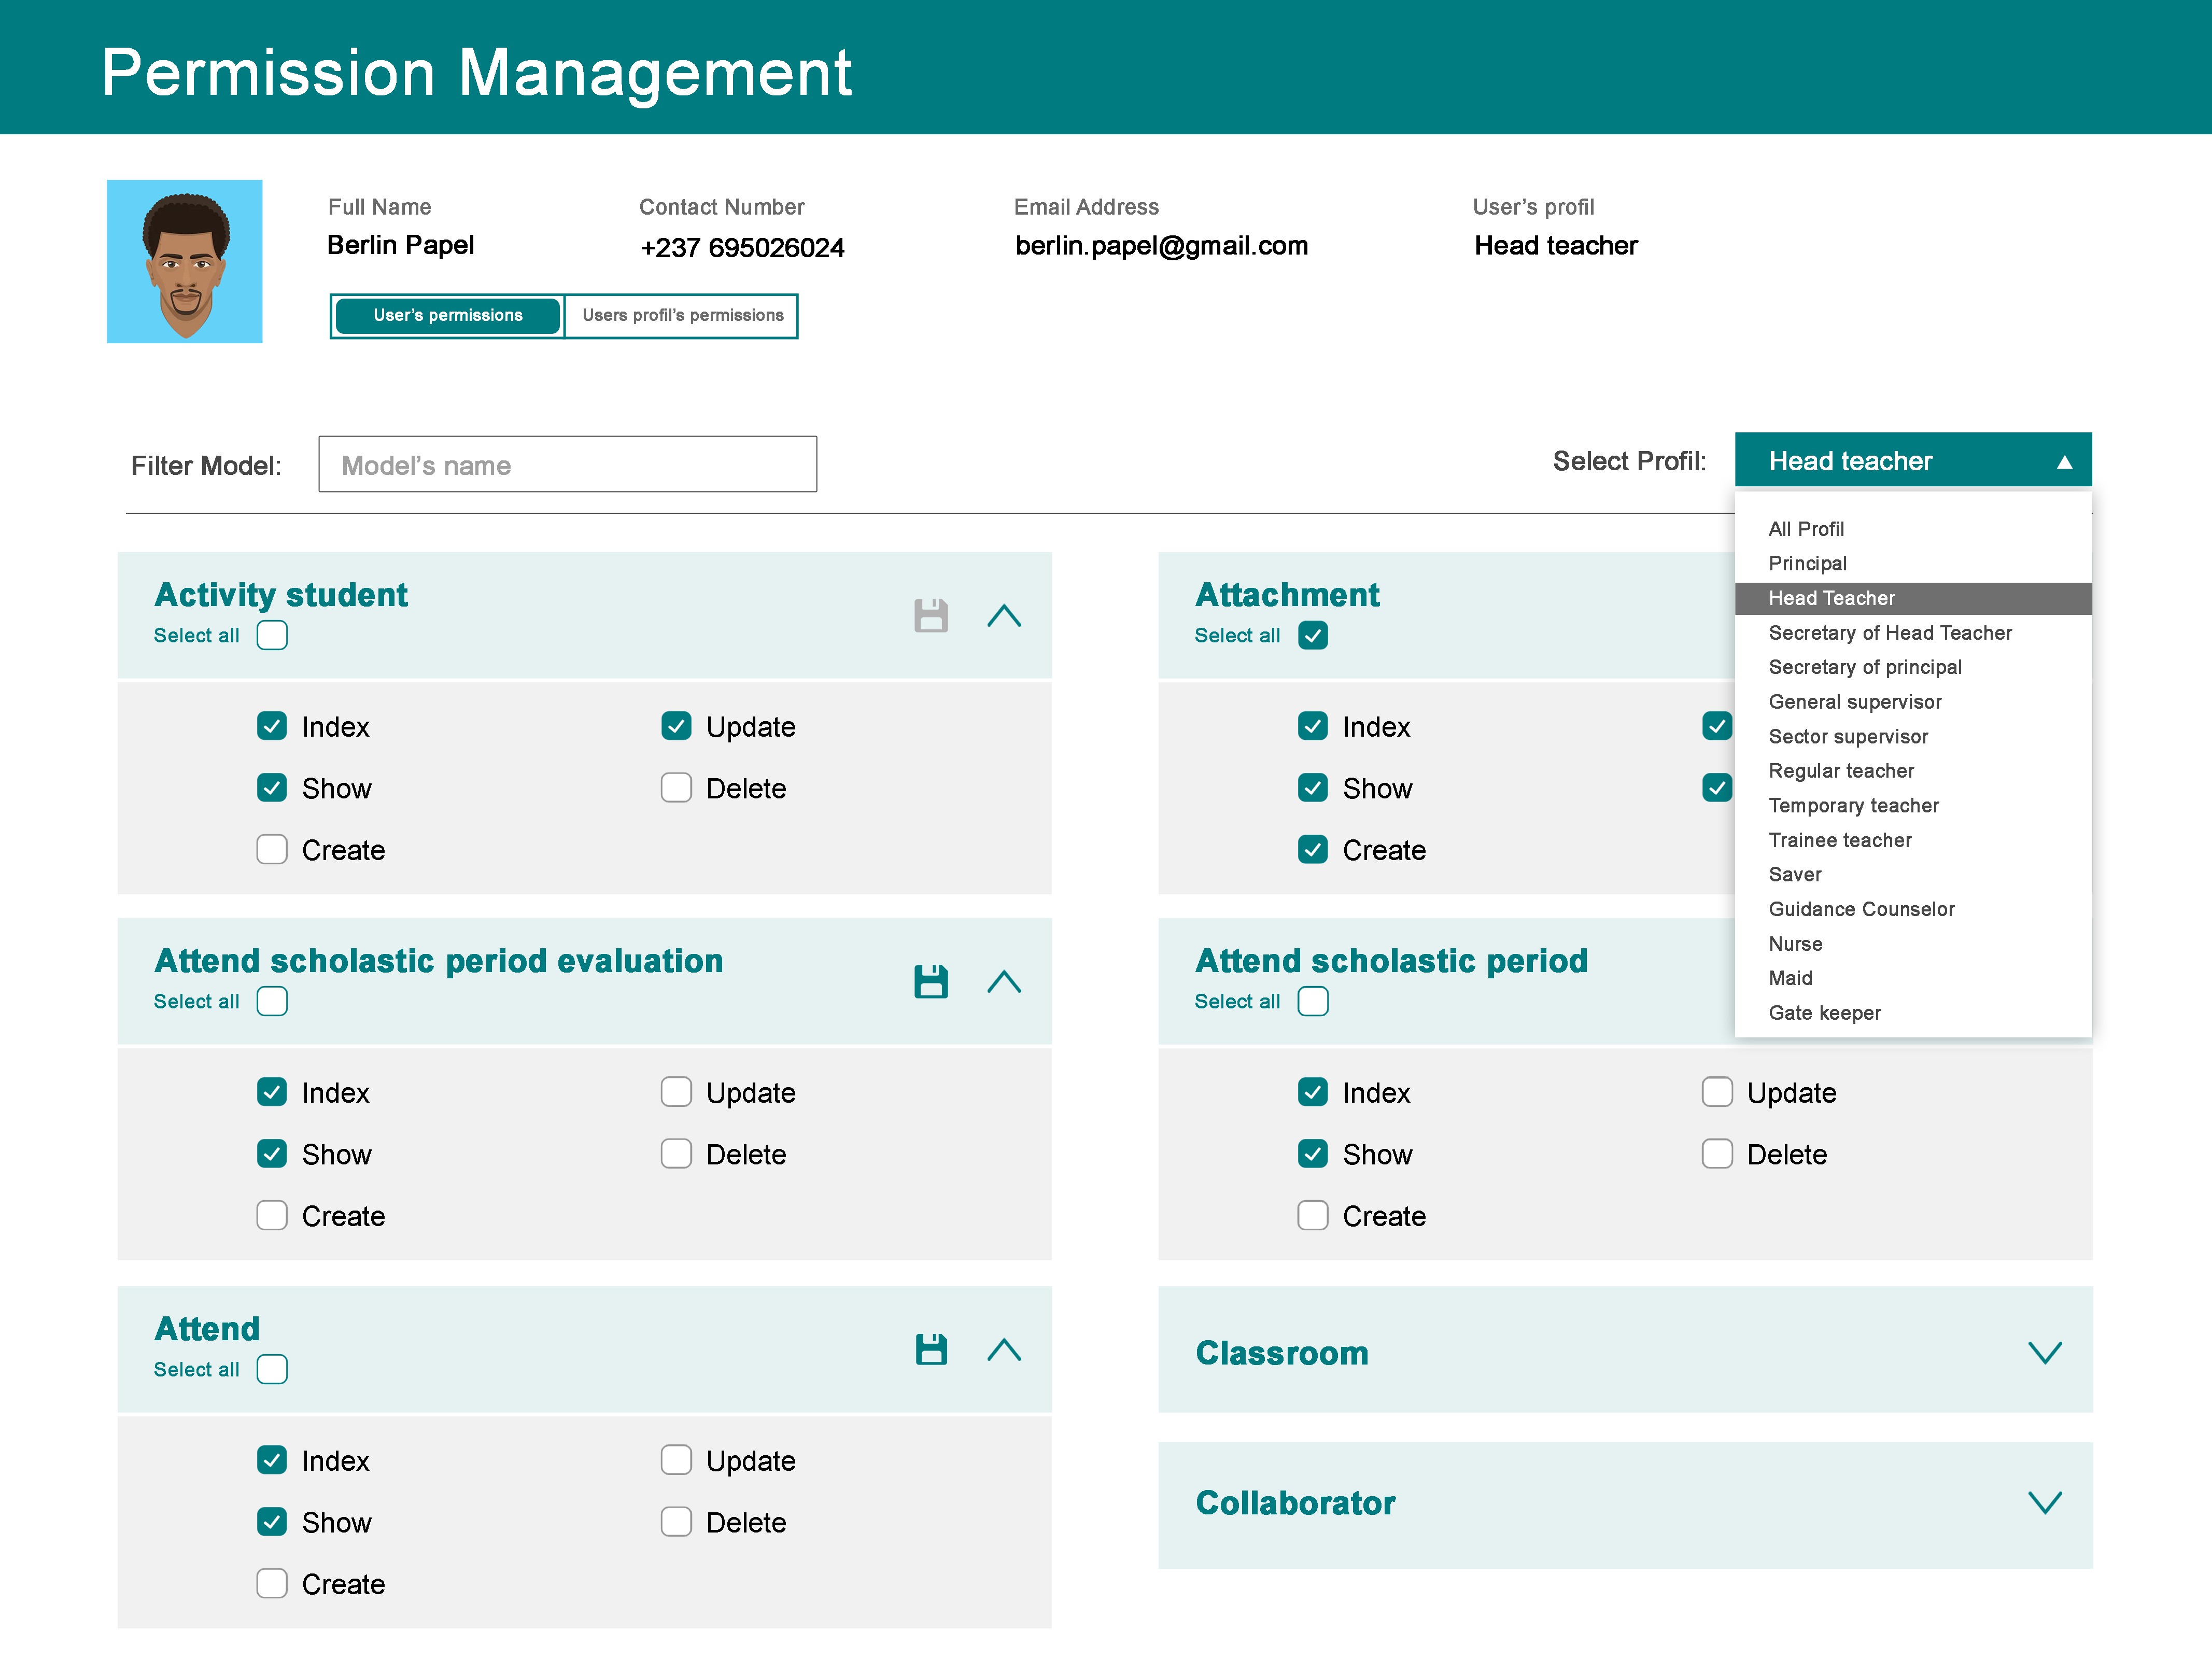
\includegraphics[width=0.8\textwidth]{../images/permission-management-desktop-mockup.jpg}
  \caption{Mockup dell'interfaccia desktop per la gestione dei permessi.}
  \label{fig:desktop-mockup}
\end{figure}

Subito sotto l'intestazione troviamo una sezione di navigazione che include due pulsanti per la
gestione dei permessi: \texttt{User's permissions} e \texttt{Users profile permissions},
che sono necessari alla selezione del tipo di permessi da gestire (quelli del singolo utente oppure
quelli del ruolo scelto).

Sotto a questi pulsanti, vi è un campo di input che permette di filtrare le risorse per nome e un menu a
tendina che consente di selezionare il profilo da modificare, con varie opzioni disponibili come \texttt{Principal,
  Secretary of Head Teacher, General Supervisor} e molte altre.

La gestione dei permessi è suddivisa in diverse risorse, come \texttt{Activity student, Attend scholastic period evaluation}
e \texttt{Attachment}, ciascuna delle quali include una serie di azioni (\texttt{Index, Show, Create, Update, Delete})
che possono essere selezionate o deselezionate dall'utente. Ogni risorsa dispone di un'opzione
\texttt{Select all} per facilitare la selezione di tutti i permessi contemporaneamente e un'icona di salvataggio
per confermare le modifiche effettuate.\\

Nella versione mobile, l'interfaccia è stata adattata per garantire un'esperienza utente ottimale su
schermi piccoli. Le informazioni dell'utente sono presentate in modo più compatto, omettendo il numero di
contatto e l'indirizzo email visibili nella versione desktop. Il titolo \texttt{Permission Management} è posizionato in alto,
accompagnato dall'avatar dell'utente.

\begin{figure}[H]
  \centering
  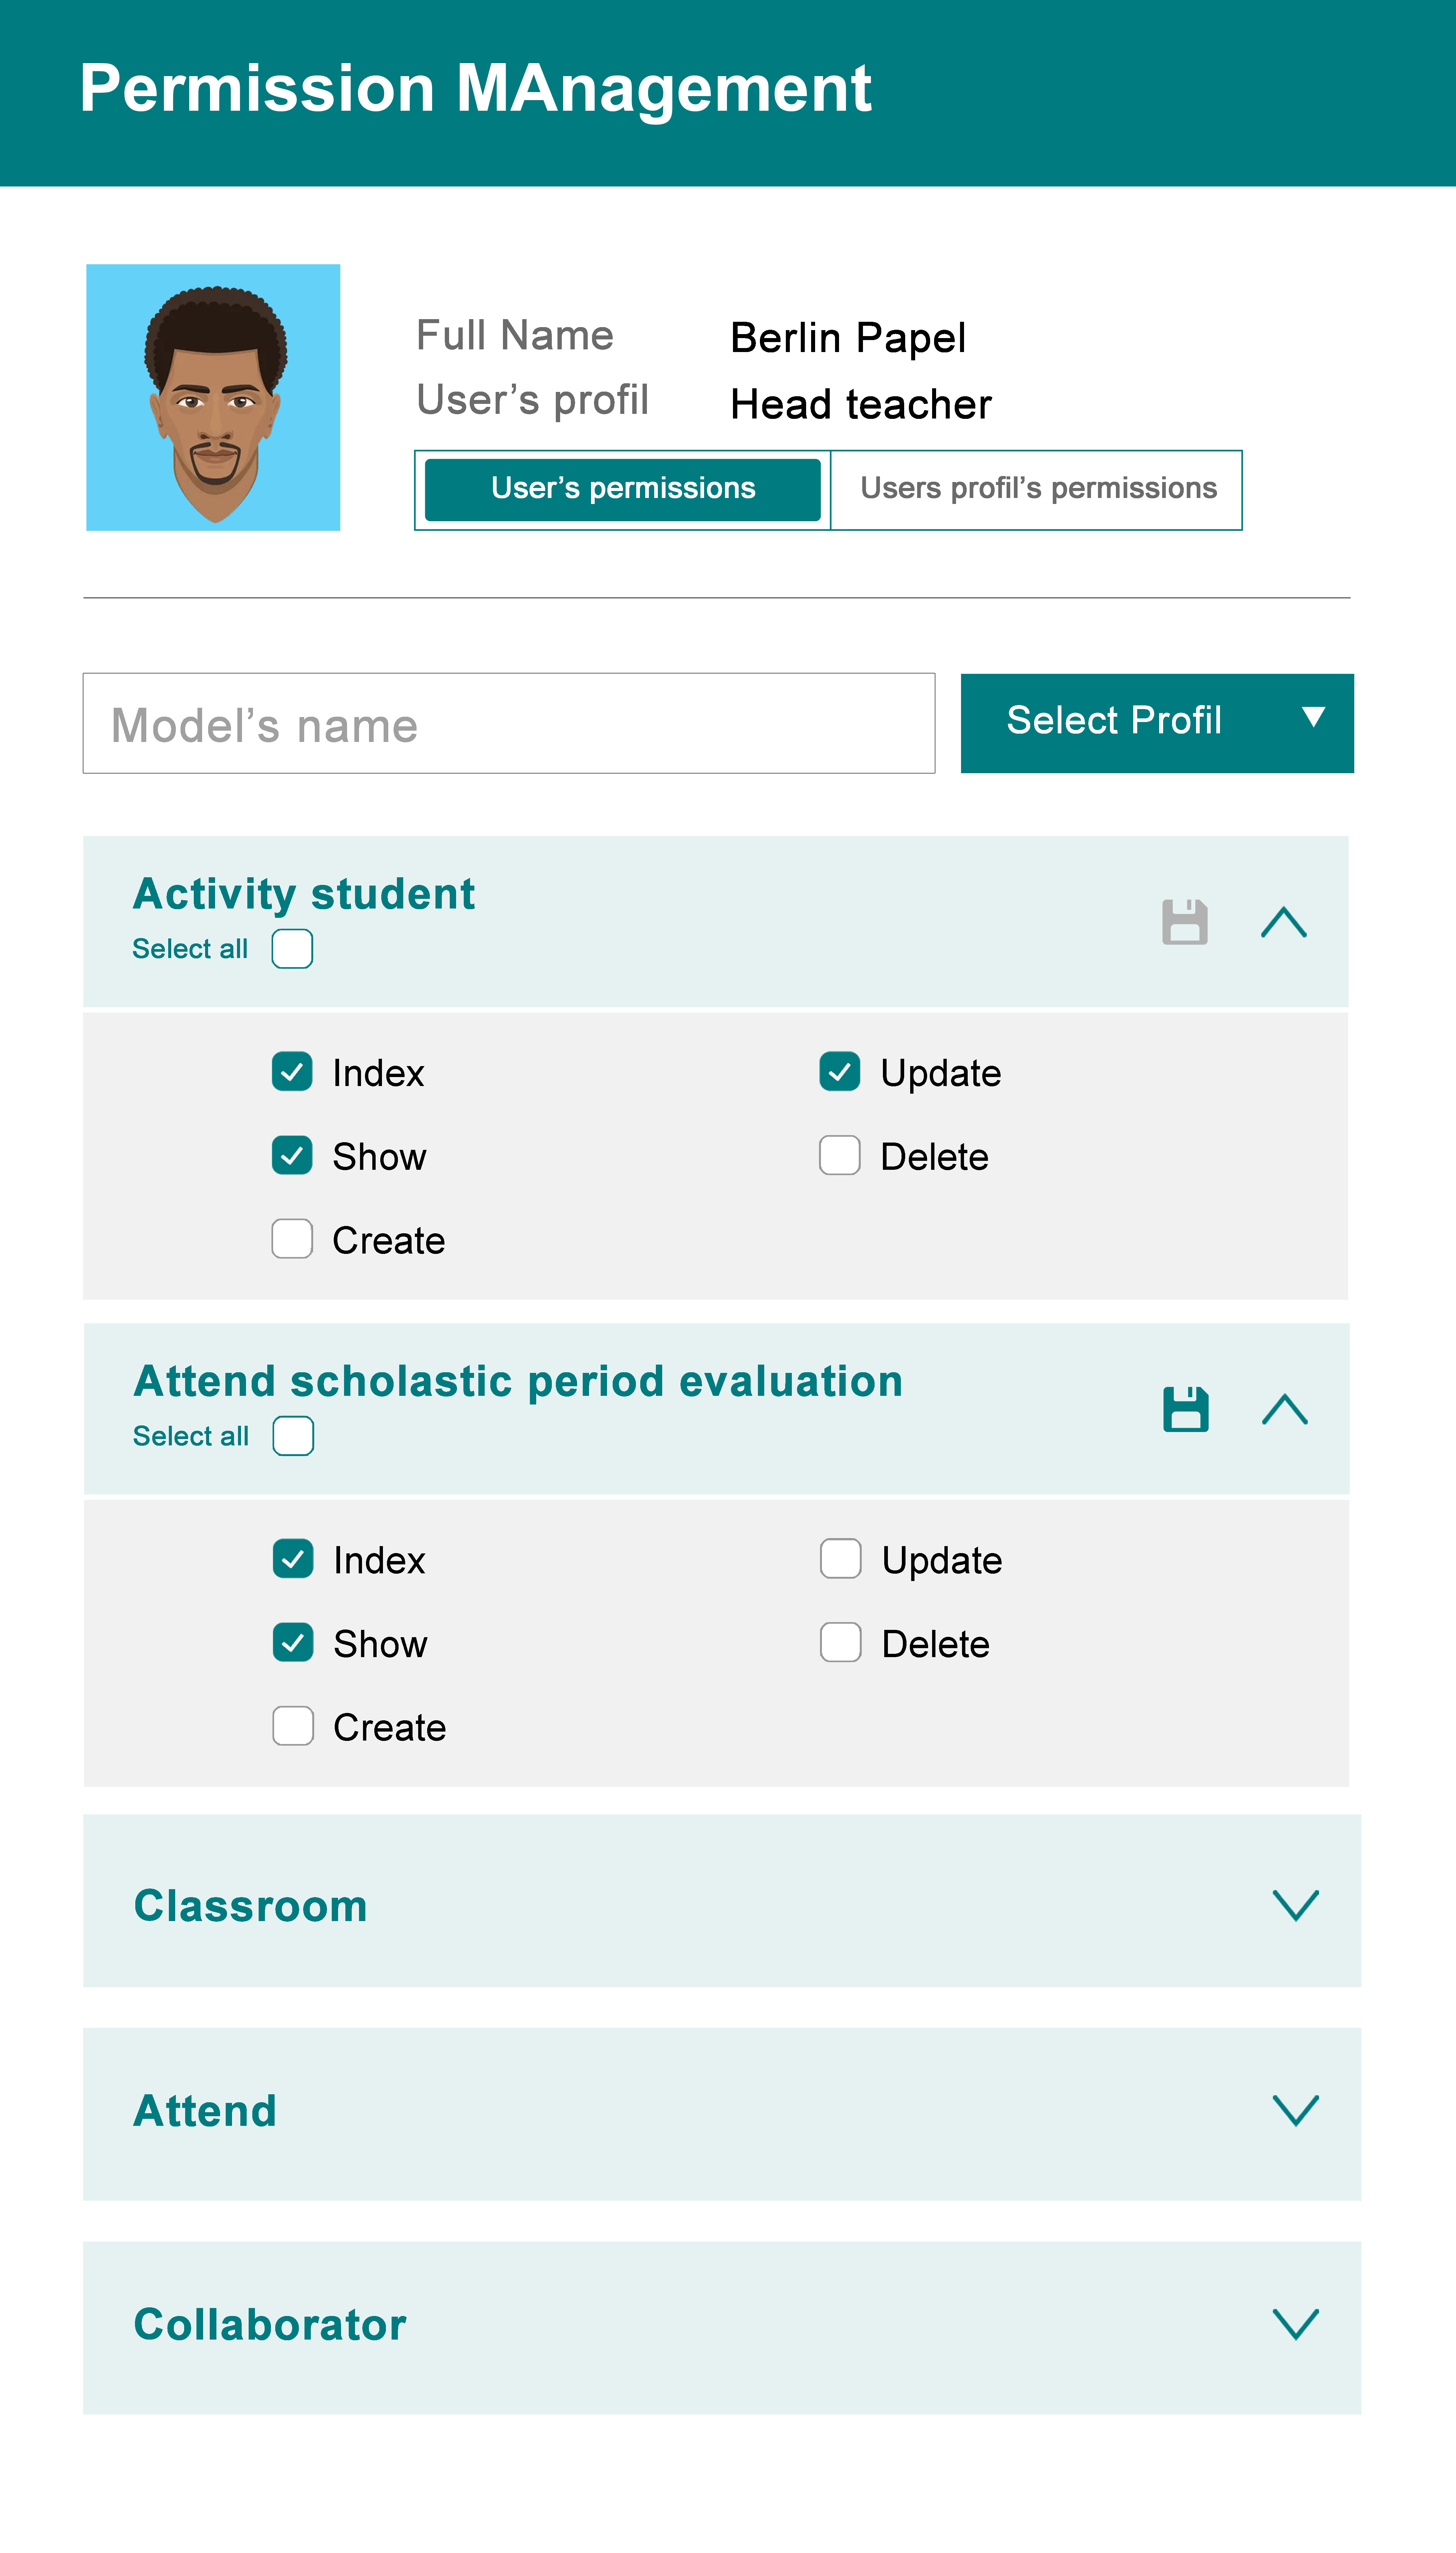
\includegraphics[width=0.4\textwidth]{../images/permission-management-mobile-mockup.jpg}
  \caption{Mockup dell'interfaccia mobile per la gestione dei permessi.}
  \label{fig:mobile-mockup}
\end{figure}

La sezione di navigazione nella versione mobile mantiene gli stessi pulsanti \texttt{User's permissions} e
\texttt{Users profile permissions}, un campo di input per filtrare i modelli per nome e un menu a tendina per la selezione
del profilo dell'utente. La gestione dei permessi in questa versione è organizzata in gruppi (di risorse) che
possono essere espansi o compressi, facilitando la navigazione. Ogni risorsa include un pulsante \texttt{Select all} e le
stesse opzioni di permessi individuali (\texttt{Index, Show, Create, Update, Delete}) presenti nella versione desktop.
Le modifiche ai permessi possono essere salvate tramite un'icona di salvataggio presente in ogni sezione.\\

Come specificato in precedenza, il design da adottare è stato inizialmente realizzato come mockup che, nel
corso del tempo e durante l'implementazione del codice, è stato modificato e rivisto in base al sorgere di
nuove esigenze.\\

Passando al design effettivo implementato per i desktop, è possibile notare come siano state apportate
diverse modifiche rispetto ai mockup iniziali.

\begin{figure}[H]
  \centering
  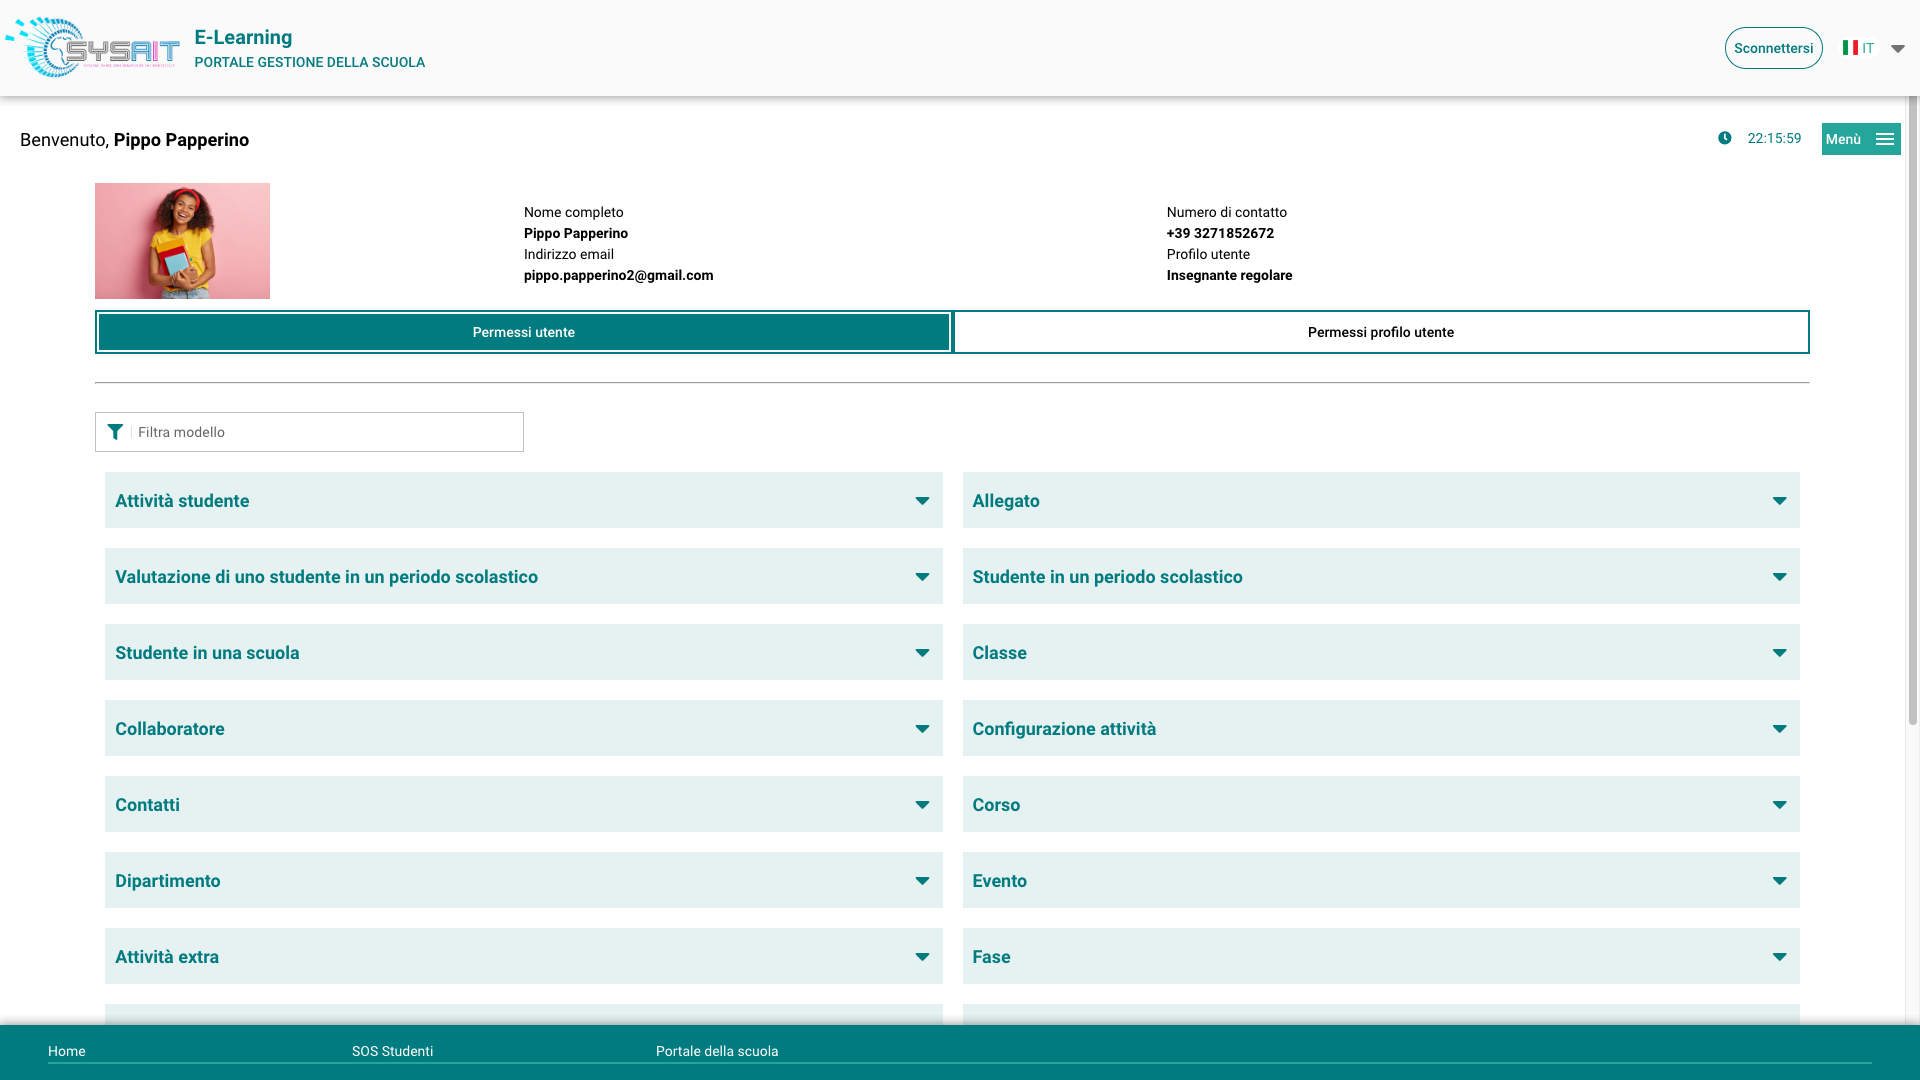
\includegraphics[width=\textwidth]{../images/permission-management-desktop.png}
  \caption{Design effettivo dell'interfaccia desktop per la gestione dei permessi.}
  \label{fig:final-desktop}
\end{figure}

Le informazioni dell'utente e il filtro delle risorse sono stati ricalcati dal mockup, mentre - per motivi di visibilità
e facilità di implementazione - i pulsanti per la selezione del tipo di permessi da gestire sono stati resi più grandi.\\

Come detto in precedenza, le modifiche apportate rispetto ai mockup originali possono essere attribuite a diversi fattori,
tra cui la necessità di migliorare l'usabilità, l'estetica, la navigabilità dell'interfaccia e, non da meno, la modalità
di implementazione (alcune scelte di design sono dipese dalla facilità di scrittura del codice necessario).\\

Discorso simile per il design effettivo dell'interfaccia mobile, che - anche in questo caso -
rispetto al mockup, vede i suddetti pulsanti per la selezione del più grandi e fruibili.

\begin{figure}[H]
  \centering
  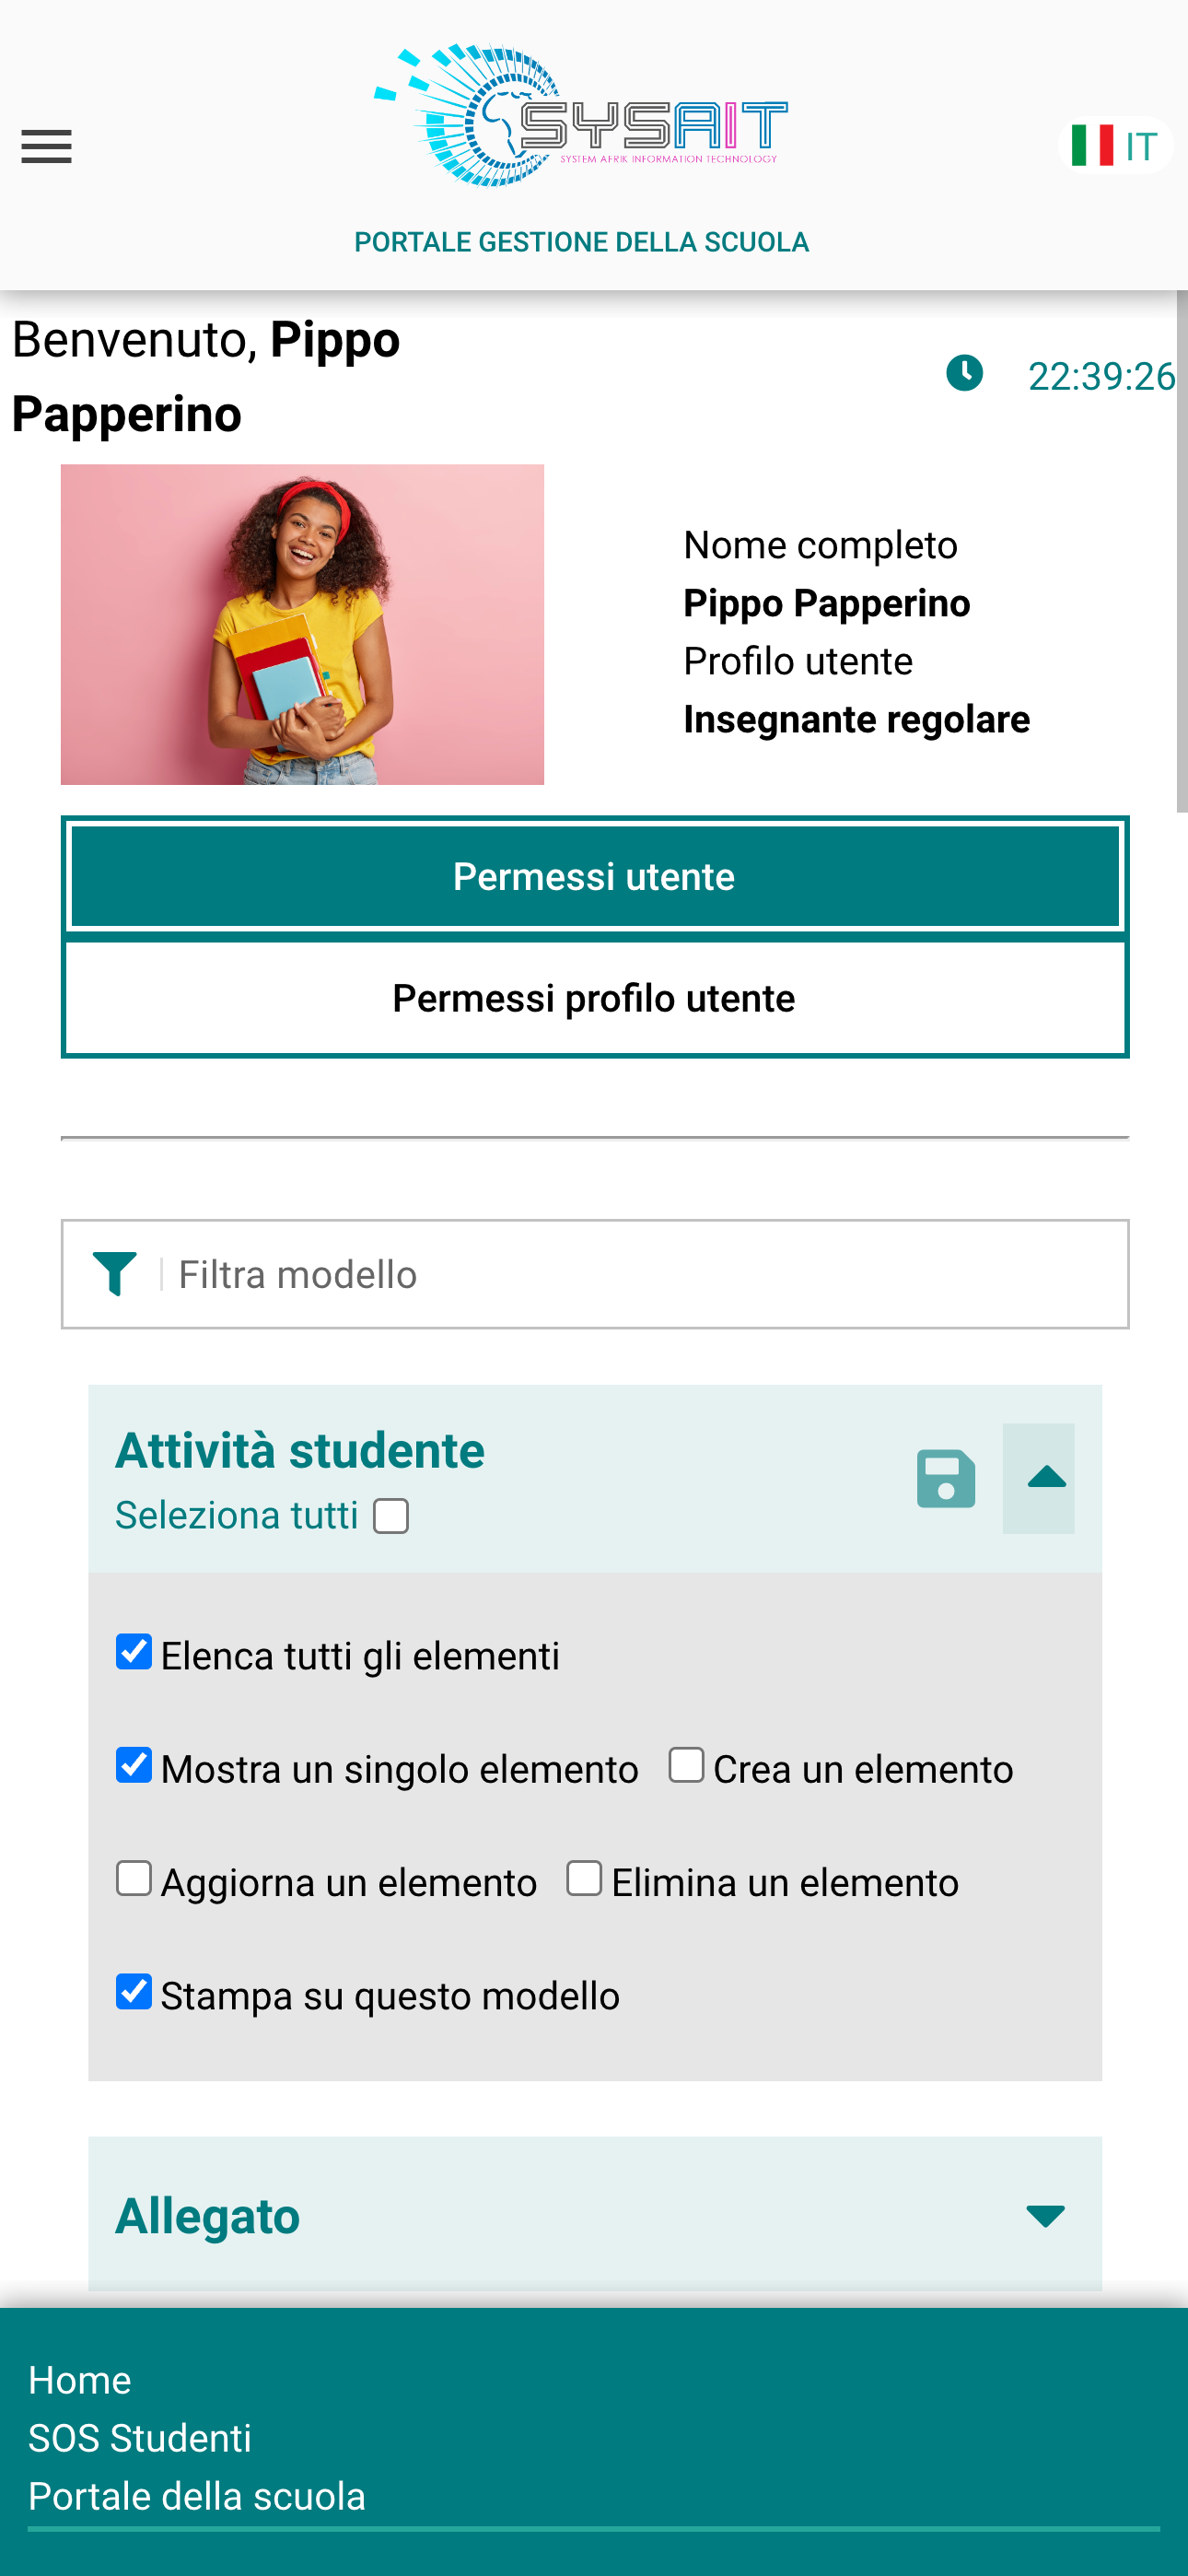
\includegraphics[width=0.4\textwidth]{../images/permission-management-mobile.png}
  \caption{Design effettivo dell'interfaccia mobile per la gestione dei permessi.}
  \label{fig:final-mobile}
\end{figure}

\newpage

\subsection{Implementazione}

Per creare l'interfaccia web per la gestione dei permessi utente sono stati utilizzati diversi componenti.
Di seguito viene descritto il componente \texttt{ButtonComponent}, che è stato utilizzato come base per creare bottoni
personalizzati nell'applicazione e, in questo caso, il pannello collassabile che poi viene utilizzato per visionare
le risorse e le relative azioni.\\

\textbf{ButtonComponent}

Il componente \texttt{ButtonComponent} realizza un bottone altamente configurabile che utilizza il framework Quasar
per Vue.js. Il suo template è mostrato nel Listing 3.1:\\

\begin{lstlisting}[language=HTML, caption=Template di ButtonComponent]
<template>
  <q-btn ... @click.prevent="handleClick">
    <slot></slot>
  </q-btn>
</template>

<script>
export default {
  name: "ButtonComponent",
  props: {
    fab: { type: Boolean, default: false },
    align: { type: String, default: "center" },
    show: { type: Boolean, default: true },
    disable: { type: Boolean, default: false },
    rounded: { type: Boolean, default: false },
    round: { type: Boolean, default: false },
    noCaps: { type: Boolean, default: false },
    padding: { type: String, default: "sm" },
    title: { type: String, default: null },
    btnClass: { type: String, default: "text-white bg-primary" },
    blank: { type: Boolean, default: false },
    size: { type: String, default: null },
    minScreen: { type: Number, default: 0 },
    to: { type: String, default: null },
    event: { type: String, default: null },
    badge: { type: String, default: null },
    badgeColor: { type: String, default: "red" },
    outline: { type: Boolean, default: false },
    label: { type: String, default: "" },
    icon: { type: String },
    iconRight: { type: String },
    flat: { type: Boolean, default: true },
    color: { type: String, default: "primary" },
    textColor: { type: String, default: "white" },
    icon_right: { type: String, default: "" },
    propStyle: { type: Object, default: null },
  },
  computed: {
    ...
  },
  methods: {
    handleClick(evt) {
      const events = {
        evt,
        event: this.event,
      };
      this.event
        ? this.$emit("click", events)
        : this.$router.push({ name: this.to });
    },
  },
};
</script>
\end{lstlisting}

Il template del componente \texttt{ButtonComponent} utilizza l'elemento \texttt{q-btn} di Quasar per creare un bottone
altamente configurabile attraverso le proprietà \texttt{props}, che permettono di modificare aspetti come
la visibilità, l'allineamento, il colore, l'icona e molto altro.\\

Il metodo \texttt{handleClick} gestisce l'evento di click sul bottone. Se viene specificato un evento \texttt{this.event},
esso viene emesso, altrimenti il bottone effettua un redirect alla pagina specificata dalla proprietà \texttt{to} del
\texttt{prop}.\\

\textbf{CollapsiblePanel}

Il componente \texttt{CollapsiblePanel} utilizza il \texttt{ButtonComponent} per creare una sezione espandibile che
può contenere altri elementi. Il Listing 3.2 mostra il codice\\

\begin{lstlisting}[language=HTML, caption=Implementazione di CollapsiblePanel]
<template>
  <div class="col WidgetWrapper" :class="`${$options.name}`">

    ...

      <div class="col-auto text-right">
        <div class="right-buttons row no-wrap">
          <div v-if="showBody">
            <ButtonComponent @click="() => $emit('buttonClick')" textColor="primary" btnClass="grey"
              v-for="(button, index) in allButtons" v-bind="button" :key="`${index}buttons`">
            </ButtonComponent>
          </div>
          <q-btn-dropdown @click="showBody = !showBody" flat></q-btn-dropdown>
        </div>
      </div>
    </div>

    ...

  </div>
</template>

<script>
import ButtonComponent from "src/components/utils/ButtonComponent.vue";

export default {
  name: "CollapsiblePanel",
  components: {
    ButtonComponent,
  },
  props: {
    title: { type: String, default: "Test Title" },
    allButtons: { type: Array, default: () => [] },
    items: { type: Array, default: () => [] },
  },
  data() {
    return { showBody: false };
  },
};
</script>
\end{lstlisting}

Il componente \texttt{CollapsiblePanel}, come detto sopra, è una sezione espandibile che può contenere altri contenuti, utilizzando
il \texttt{ButtonComponent} per creare bottoni che possono essere cliccati per eseguire azioni specifiche.\\

\textbf{PermissionCollapsiblePanel}

Il componente \texttt{PermissionCollapsiblePanel} estende \texttt{CollapsiblePanel} per gestire i permessi
degli utenti. Il codice è mostrato nel Listing 3.3:\\

\begin{lstlisting}[language=HTML, caption=Implementazione di PermissionCollapsiblePanel]
<template>
  <div :class="`${$options.name} row`" class="collapsible-panel-container">
    <CollapsiblePanel :title="panel.title" :allButtons="allButtons" class="collapsible-panel" style="padding: 10px"
      @buttonClick="saveProcess">
      <template v-slot:subtitle-slot>
        <label style="display: flex">{{ $t('selectAll') }} <input type="checkbox" style="margin-left: 5px"
            v-model="selectAll" /></label>
      </template>
      <template v-slot:content-body>
        <div class="row elements">
          <div v-for="(item, index) in panel.items" :key="index" class="checkbox">
            <label>
              <input class="single-element" type="checkbox" v-model="item.checked" @change="updateChanges" />
              {{ $t(`${item.label}`) }}
            </label>
          </div>
        </div>
      </template>
    </CollapsiblePanel>
  </div>
</template>

<script>
import CollapsiblePanel from "src/components/permissions/CollapsiblePanel.vue";

export default {
  name: "PermissionCollapsiblePanels",
  components: { CollapsiblePanel },
  props: {
    panel: { type: Object, default: () => { } },
  },
  data() {
    return {
      allButtons: [{ icon: "fas fa-save", event: 'save', disabled: true }],
      changesMade: false,
    };
  },
  computed: {
    selectAll: {
      ...
    }
  },
  methods: {
    selectAllItems(value) {
      ...
    },
    allItemsChecked() {
      return this.panel.items.every(item => item.checked)
    },
    ...
    saveProcess() {
      let permissions = {};

      for (let item of this.panel.items) {
        permissions[item.label] = item.checked;
      }

      this.$emit('updatePermissions', { permissions, model: this.panel.model });

      ...

    }
  }
};
</script>
\end{lstlisting}

Il componente \texttt{PermissionCollapsiblePanel} aggiunge la gestione dei permessi, includendo
una lista di checkbox (le azioni) che rappresentano i permessi, con un'opzione per selezionare tutti i permessi
tramite una checkbox globale, e il pulsante per salvare le modifiche fatte.\\

Il metodo \texttt{saveProcess} raccoglie lo stato dei permessi e lo invia tramite l'evento \texttt{updatePermissions}.\\

\textbf{Permission Collapsible Panels}

Infine, il componente \texttt{PermissionCollapsiblePanels} utilizza \\ \texttt{PermissionCollapsiblePanel} per
visualizzare più pannelli di permessi. Ecco il codice:\\

\begin{lstlisting}[language=HTML, caption=Implementazione di PermissionCollapsiblePanels]
<template>
  <div :class="`${$options.name} row`" class="collapsible-panel-container">
    <PermissionCollapsiblePanel v-for="(panel, index) in panels" :key="`${index}panels`" :panel="panel"
      @updatePermissions="(params) => $emit('updatePermissions', params)" class="col-md-6 col-12">
    </PermissionCollapsiblePanel>
  </div>
</template>

...
\end{lstlisting}

Ogni volta che vengono aggiornati i permessi in uno dei pannelli, l'evento \texttt{updatePermissions} viene
emesso per informare il componente padre dei cambiamenti.\\

\textbf{Permissions.vue}

Il componente \texttt{Permissions.vue}, ossia la pagina che l'utente visualizza e di cui il design è stato mostrato
nell'apposito capitolo, utilizza \texttt{PermissionCollapsiblePanels} per fornire un'interfaccia completa per
la gestione dei permessi utente. Ecco il codice:\\

\begin{lstlisting}[caption=Implementazione di Permissions.vue]
<template>
  <div class="page-container" :class="`${$options.name}`">
    <q-page :class="`${$options.name}`">
      <div class="permissions" style="margin: 0 5%">
        <div class="row permissions-user-infos items-center" v-if="userId && isUserDataLoaded">

          ...

          <div class="permission-buttons-col col-12">
            <div class="row permission-type-buttons">
              <ButtonComponent class="user-permissions-button col-12 col-md-6" v-bind="userPermissionsProp"
                @click="handleUserPermissionsSelection" />
              <ButtonComponent class="user-profile-permissions-button col-12 col-md-6"
                v-bind="userProfilePermissionsProp" @click="handleUserProfilePermissionsSelection" />
            </div>
          </div>
        </div>

       ...

        <div class="row permissions-filters items-center">
          <div class="col-md-3 col-12">
            <InputComponent class="filter-model" :options="panels" v-bind="filterProps" @updated="handleModelSearch" />
          </div>
          <!-- Selection of profile, only visible if there is no userId -->
          <div class="col-md-4 col-12 offset-md-5">
            <div v-if="profileOptions.length > 0 && !userId">
              <InputComponent class="profile-selection" :options="profileOptions" v-bind="selectProps"
                @updated="handleProfileSelection" />
            </div>
          </div>
        </div>

        <div class="row permissions-actions" :key="`${showPanels}showPanels`" v-if="showPanels">
          <div v-if="noModelFound">
            <b>{{ this.$t(`noModelFound`) }}</b>
          </div>
          <div v-else>
            <PermissionCollapsiblePanels :panels="filteredPanels" @updatePermissions="updatePermissions" />
          </div>
        </div>
      </div>
    </q-page>
  </div>
</template>

<script>
...

export default {
  name: "Permissions",
  mixins: [checkingDependencyOfModels],
  components: {
    PermissionCollapsiblePanels,
    InputComponent,
    ButtonComponent,
  },
  data() {
    return {
      permissionsParams: {},
      panels: [],
      filteredPanels: [],
      userId: this.$route.params.userId,
      schoolId: this.$route.params.schoolId,
      userData: [],
      profileOptions: [],
      selectedProfile: null,
      noModelFound: false,
      selectProps: {
        isSelect: true,
        isRequired: true,
        mapOptions: true,
        emitValue: true,
        prependIcon: "fas fa-user",
        name: "profile",
        useInput: false,
        clearable: true,
        label: this.$t(`selectProfile`),
        outlined: true
      },
      filterProps: {
        prependIcon: "fas fa-filter",
        name: "filter",
        useInput: true,
        clearable: true,
        label: this.$t(`filterModel`),
        maxlength: 60,
        outlined: true
      },
      userPermissionsButtonIsSelected: true,
      userPermissionsProp: {
        label: this.$t(`userPermissions`),
        noCaps: true,
        event: 'handleUserPermissionSelection',
        btnClass: 'bg-primary',
        textColor: 'white',
      },
      userProfilePermissionsProp: {
        ...
      }
    };
  },

  ...

  },

  mounted() {
    this.fetchProfiles();
    this.fetchModels();
    this.fetchUserData();
    this.permissionsButtonSelection();
  },
  methods: {
    async updatePermissions(permissionsParams) {
      this.permissionsParams = { ...permissionsParams };
      try {
        const savedPermissions = await this.$hs.methods.ajaxCall(`/users/edit_permissions`, "patch", { params: this.form });
        // console.log("Edited permissions: ", savedPermissions);
      } catch (error) {
        console.error("Error updating permissions: ", error);
      }
    },
    async fetchModels() {
      if (this.isUserPermissions) {
        // If there's an userId, get user's permissions and models here
        try {
          const permissionsResp = await this.$hs.methods.ajaxCall(`/users/permissions?user_id=${this.userId}`, "get");
          // Transformation of the object into an array of panel objects
          this.panels = Object.entries(permissionsResp.data.permissions).map(([title, permissions]) => ({
            title: this.$t(`permissions.${title}`),
            model: title,
            items: Object.entries(permissions).map(([label, checked]) => ({
              label,
              checked
            }))
          }));
          this.filteredPanels = this.panels;
        } catch (error) {
          console.error("Error fetching user permissions: ", error);
        }
      }
    },
    async fetchProfiles() {
      if (!this.userId) {
        try {
          const profilesResp = await this.$hs.methods.ajaxCall(`/profiles?minimal=true`, "get");
          this.profileOptions = profilesResp.data;
        } catch (error) {
          console.error("Error fetching profiles: ", error);
        }
      }
    },
    async fetchUserData() {
      if (this.userId) {
        try {
          const userDataResp = await this.$hs.methods.ajaxCall(`/users/user_home?user_id=${this.userId}`, "get");
          this.userData = userDataResp.data;
        } catch (error) {
          console.error("Error fetching user data: ", error);
        }
      }
    },
    ...
  }
}

...
\end{lstlisting}

Questa complessa pagina, costituita da varie chiamate al backend che gestiscono i dati
degli utenti (la loro ricezione e la loro visualizzazione), il caricamento dei loro permessi e la modifica degli stessi, fa
ampio uso dei componenti sopra descritti e dei relativi \texttt{prop} per personalizzarli e renderli funzionali allo scopo
del progetto.

\newpage

%%% ---- FINE CORPO 'FRONTEND' -----

%%% ---- CORPO 'BACKEND' -----

\section{Gestione backend dei permessi}

\subsection{Schema del DB}

Il progetto, come già detto, utilizza \texttt{PostgreSQL} come sistema di gestione di database relazionali, mentre per
visualizzare e amministrare il database in modo efficace viene utilizzato \texttt{pgAdmin 4}, programma dotato
di un'interfaccia grafica potente e intuitiva che facilita la gestione delle strutture del database,
l'esecuzione di query SQL e l'analisi dei dati.\\

A proposito della struttura del database, si rende ora necessario definire il diagramma ERD (\texttt{Entity-Relationship Diagram}),
e lo schema relazionale, al fine di avere una panoramica complessiva della parte di DB relativa ai permessi utente.\\

\textbf{Diagramma Entità-Relazione (\texttt{ERD})}

Per modellare le relazioni tra le entità coinvolte nella gestione dei permessi, è possibile utilizzare
un diagramma entità-relazione (\texttt{ERD}, \texttt{Entity-Relationship Diagram}). Questo diagramma mostra come
le entità "Serves", "User" e "School" siano correlate tra loro.\\

\begin{figure}[H]
  \centering
  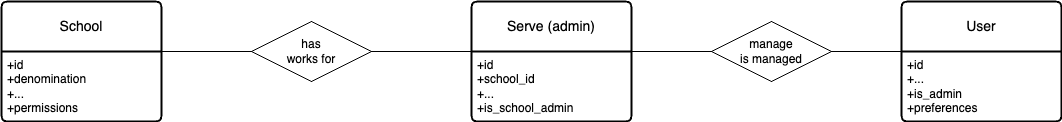
\includegraphics[width=\textwidth]{../images/diagramma-erd.png}
  \caption{Diagramma ERD per la gestione dei permessi}
\end{figure}

\textbf{Tabella users}

La tabella users rappresenta gli utenti dell'applicazione. Di seguito vengono descritti i campi principali:

\begin{itemize}
  \item \textbf{id}: Identificatore unico per ogni utente;
  \item \textbf{email}: Indirizzo email dell'utente;
  \item \textbf{first\_name}: Nome dell'utente;
  \item \textbf{last\_name}: Cognome dell'utente;
  \item \textbf{is\_admin}: Booleano che indica se l'utente ha privilegi amministrativi;
  \item \textbf{userable\_type}: Tipo di entità collegata all'utente (ad es. "Staff" o "Student");
  \item \textbf{userable\_id}: ID dell'entità collegata all'utente;
  \item \textbf{identification\_number}: Numero identificativo univoco dell'utente;
  \item \textbf{preferences}: Preferenze specifiche relative alla scuola preferita dell'utente in formato JSON;
  \item \textbf{avatar\_url}: URL dell'immagine avatar dell'utente;
\end{itemize}

\textbf{Tabella schools}

La tabella \texttt{schools} rappresenta le scuole gestite dall'applicazione. Di seguito vengono descritti i campi principali:

\begin{itemize}
  \item \textbf{id}: Identificatore unico per ogni scuola;
  \item \textbf{denomination}: Nome ufficiale della scuola;
  \item \textbf{contacts\_info}: Informazioni di contatto della scuola in formato JSON (email, indirizzo, numeri di
        telefono);
  \item \textbf{social\_media}: Informazioni sui social media della scuola in formato JSON (URL dei profili social);
  \item \textbf{identification\_number}: Numero identificativo univoco della scuola;
  \item \textbf{theme\_id}: ID del tema grafico associato alla scuola;
  \item \textbf{root\_id}: ID della scuola radice nel caso di un'organizzazione gerarchica;
  \item \textbf{parent\_id}: ID della scuola genitore nel caso di un'organizzazione gerarchica;
  \item \textbf{category\_id}: ID della categoria della scuola;
  \item \textbf{permissions}: Permessi dei profili associati alla scuola in formato JSON;
\end{itemize}

\textbf{Tabella serves}

La tabella \texttt{serves} rappresenta il collegamento tra il personale (staff) e le scuole.
Di seguito vengono descritti i campi principali:

\begin{itemize}
  \item \textbf{id}: Identificatore unico per ogni record;
  \item \textbf{school\_id}: ID della scuola a cui il personale è assegnato;
  \item \textbf{job\_id}: ID del lavoro specifico del personale (può essere nullo);
  \item \textbf{profile\_id}: ID del profilo del personale;
  \item \textbf{departement\_id}: ID del dipartimento del personale (può essere nullo);
  \item \textbf{first\_serving\_date}: Data di inizio del servizio del personale nella scuola;
  \item \textbf{is\_school\_admin}: Boleano che indica se il personale è amministratore della scuola.
\end{itemize}

A conclusione di questa sezione, si riporta lo schema relazionale dei dati finora descritti:

\begin{figure}[H]
  \centering
  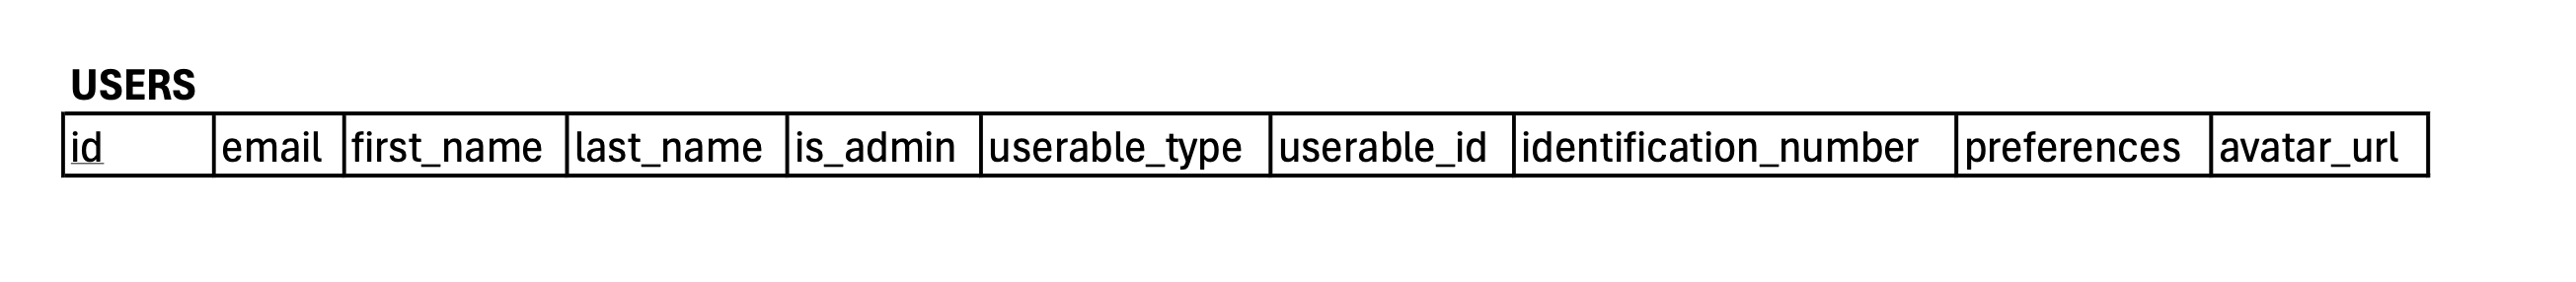
\includegraphics[width=\textwidth]{../images/schema-relazionale-users.png}
  \caption{Schema relazionale di Users}
\end{figure}

\begin{figure}[H]
  \centering
  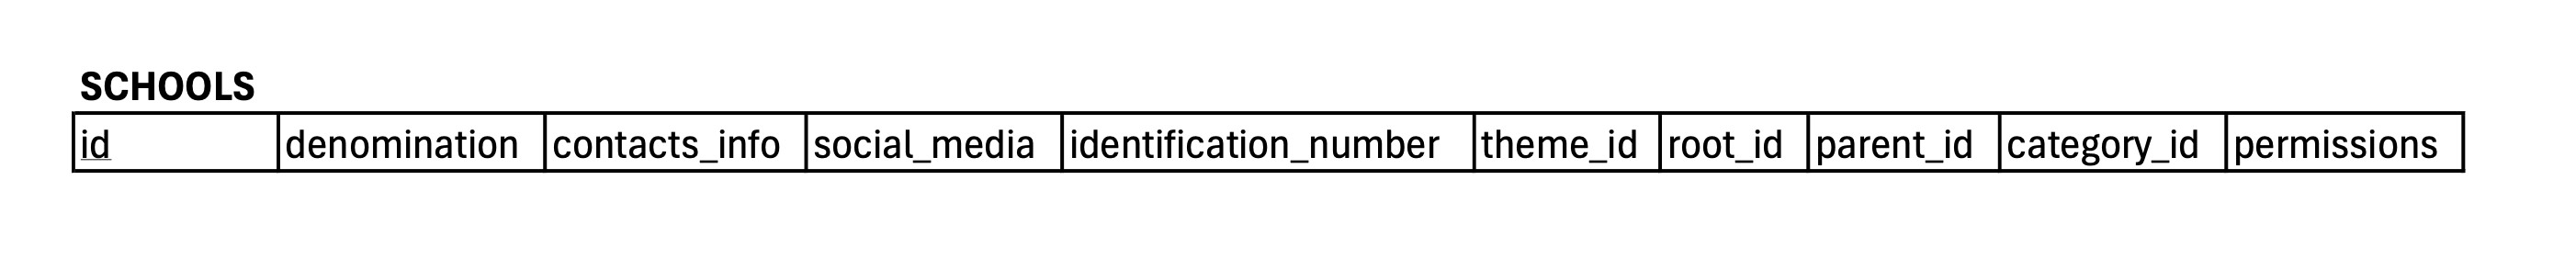
\includegraphics[width=\textwidth]{../images/schema-relazionale-schools.png}
  \caption{Schema relazionale di Schools}
\end{figure}

\begin{figure}[H]
  \centering
  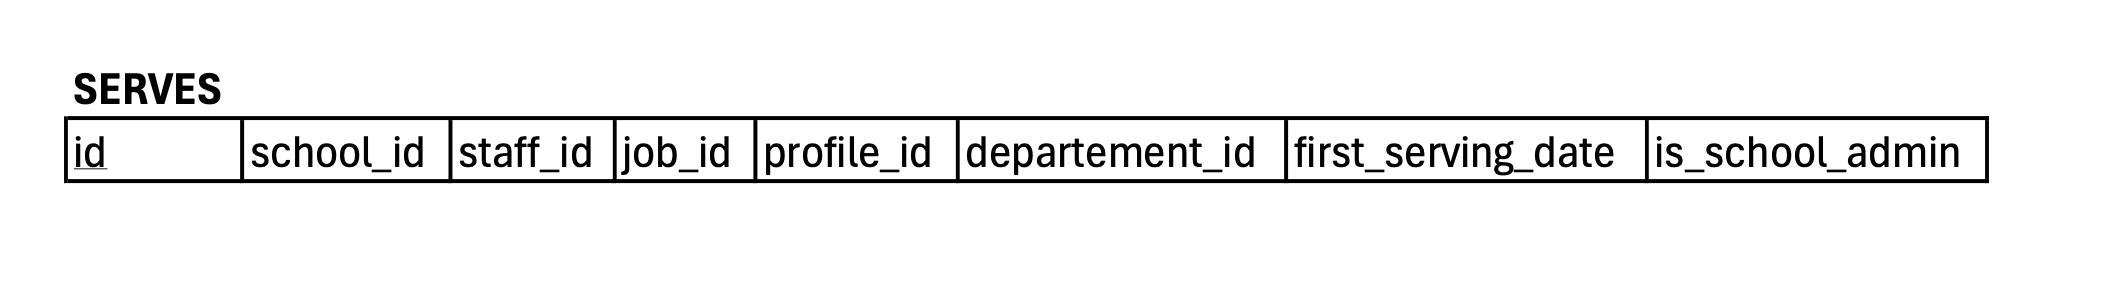
\includegraphics[width=\textwidth]{../images/schema-relazionale-serves.png}
  \caption{Schema relazionale di Serves}
\end{figure}

In tutti e tre i casi, \texttt{id} è la chiave primaria.

\newpage

\subsection{Inizializzazione del database}

Il progetto di tirocinio, oggetto di questa tesi, è stato sviluppato principalmente utilizzando per il backend il linguaggio
di programmazione Ruby e il framework Ruby on Rails.\\

Per poter testare ed utilizzare la piattaforma sul proprio dispositivo di sviluppo, è stato ovviamente necessario
inizializzare il database e, più in generale, l'intero backend: per fare ciò, sono state sfruttate le pagine presenti su
Confluence e appositamente realizzate per permettere un veloce ed efficace onboarding di nuovi membri del team di sviluppatori
e tirocinanti.\\

Per avviare il progetto, è stato innanzitutto necessario installare Ruby e Ruby on Rails nell'ambiente di sviluppo che, nel caso
dello scrivente, è MacOS su hardware utilizzante architettura ARM. Questo dettaglio viene specificato perchè ciò ha richiesto
delle fasi aggiuntive di \texttt{troubleshooting} che hanno reso il processo di inizializzazione del progetto leggermente più
tedioso di quando viene utilizzato un dispositivo dotato di processore con architettura x64 o x84.\\

Dopo aver risolto le problematiche causate dall'architettura ARM ed aver installato strumenti fondamentali come Visual Studio
Code (già adoperato per vari insegnamenti del corso di studi) e qualche estensione per facilitare la scrittura del codice (come,
ad esempio, \texttt{Auto Close Tag} per automatizzare la chiusura dei tag HTML/XML, \texttt{Beautify css/sass/less} per
formattare automaticamente il codice CSS per renderlo più leggibile e coerente e \texttt{Bracket Pair Colorizel} per assegnare
colori diversi alle coppie di parentesi corrispondenti), si è proceduto con la creazione di un account Bitbucket che, come
descritto prima, è il sito su cui è stato caricato il progetto e con cui, grazie a Git, si sono sviluppate le funzionalità
richieste ed è stato condiviso il codice.\\

A seguito della creazione dell'account, è stato necessario configurare \texttt{SSH (Secure Shell)}, protocollo sicuro
di accesso remoto che consente di stabilire connessioni sicure tra computer su una rete non protetta come Internet. Alcuni
dei vantaggi dell'utilizzo di SSH per interagire con Bitbucket, rispetto alle semplici credenziali HTTPS, è quello di
utilizzare coppie di chiavi crittografiche eliminano la necesità di inserire ripetutamente la password e, conseguentemente,
offrire una maggiore sicureza ed automatizzare attività come il psuh e il pull del codice. Ciò è particolarmente utile in
scenari di integrazione continua e deployment continuo (\texttt{CI/CD}).\\

Per configurare la connessione SSH sono stati eseguiti i seguenti comandi, che hanno prodotto la chiave pubblica
\texttt{id\_rsa.pub} che poi è stata caricata nelle impostazioni dell'account BitBucket:\\

\begin{lstlisting}[language=bash, caption=Generazione della chiave SSH]
  ssh-keygen
  ssh-add ~/.ssh/id_rsa
  \end{lstlisting}

Dopo l'inizializzazione della chiave SSH, si è proceduto con l'installazione di Ruby nella sua versione 3.0.2 e di Ruby
on Rails 6.1.4, per poi proseguie con PostgreSQL e pgAdmin (strumento importante avere una GUI -  Graphic User Interface -
da cui poter vedere rapidamente il database del progetto).\\

A tutto ciò è seguita la clonazione dalla repository remota di BitBucket della piattaforma di E-learning sul dispositivo locale
e la creazione di un file di testo semplice \texttt{.env} che contiene variabili d'ambiente. Queste variabili sono
coppie chiave-valore che memorizzano informazioni di configurazione come chiavi API, password del database, URL di
servizi esterni e altre impostazioni specifihe dell'ambiente in cui l'applicazione viene eseguita.\\

Una volta terminata la realizzazione del file \texttt{.env}, sono state installate le dipendenze di progetto (chiamate
\texttt{gemme} o \texttt{gems} in Ruby, pacchetti di codice che aggiungono funzionalità) e \texttt{bundler}, strumento che
facilità la gestione delle suddette dipendenze sfruttando un file chiamato \texttt{Gemfile},
contente l'elenco di tutte le gemme di cui il progetto ha bisogno.\\

A questo punto si è arrivati alla fase effettiva di inizializzazione del database locale con il comando

\begin{lstlisting}[language=ruby, caption=Inizializzazione del DB locale]
  rails db:create
  \end{lstlisting}

E la creazione delle tabelle con

\begin{lstlisting}[language=ruby, caption=Creazione tabelle]
  rails db:migrate
  rails db:migrate RAILS_ENV=test
  \end{lstlisting}

Ed infine

\begin{lstlisting}[language=ruby, caption=Avviamento del progetto]
  rails server -p 3002
  \end{lstlisting}

Per eseguire l'applicativo in un web browser.

\newpage

\subsection{Implementazione}

Prima di parlare dell'effettiva implementazione del modulo di gestione dei permessi utente, occorre descrivere alcune gemme
fondamentali: \texttt{Devise}, \texttt{Pundit} e \texttt{Rolify}. Di seguito verranno illustrate le caratteristiche principali
di ciascuna gemma e le modalità di utilizzo nel contesto dell'applicazione.\\

\textbf{Devise}

Devise \cite{Devise} è una gemma per Ruby on Rails che facilita la gestione dell'autenticazione
degli utenti. Fornisce un set completo di moduli per gestire tutte le funzionalità legate all'autenticazione,
come registrazione, login, recupero password, conferma dell'email, ecc.\\

\textbf{Caratteristiche principali}:

\begin{enumerate}
  \item \textbf{Autenticazione}: gestisce il login e la registrazione degli utenti;
  \item \textbf{Recupero password}: permette agli utenti di recuperare la password dimenticata;
  \item \textbf{Conferma account}: invia email di conferma per la verifica dell'account;
  \item \textbf{Timeout}: gestisce la scadenza delle sessioni degli utenti inattivi.
\end{enumerate}

Di seguito i comandi rilevanti per utilizzare la gemma:\\

\begin{lstlisting}[language=ruby, caption=Utilizzo di Devise]
  gem 'devise'                  # Aggiunta gemma al 'Gemfile'
  bundle install                # Installazione della gemma
  rails generate devise:install # Configurazione di Devise
  rails generate devise User    # Generazione modello User
  rails db:migrate              # Esecuzione delle migrazioni
  \end{lstlisting}

\newpage

Devise aggiunge automaticamente le rotte necessarie per l'autenticazione. Nel file config/routes.rb:\\

\begin{lstlisting}[language=ruby, caption=Configurazione delle rotte]
    Rails.application.routes.draw do
      devise_for :users
      # Altre rotte
    end
    \end{lstlisting}

\textbf{Pundit}

Pundit \cite{Pundit} è una gemma per la gestione delle autorizzazioni in un'applicazione Ruby on Rails.
Utilizza una combinazione di plain Ruby e oggetti policy per autorizzare le azioni degli utenti.\\

\textbf{Caratteristiche principali}:
\begin{enumerate}
  \item \textbf{Policy}: ogni modello ha una policy associata che definisce chi può fare cosa.
  \item \textbf{Scopes}: controllano quali record un utente può vedere.
  \item \textbf{Facile integrazione}: si integra facilmente con i controller di Rails.
\end{enumerate}

I comandi per utilizzarla sono simili a quelli di Devise:\\

\begin{lstlisting}[language=ruby, caption=Utilizzo di Pundit]
  gem 'pundit'                  # Aggiunta gemma al 'Gemfile'
  bundle install                # Installazione della gemma
  rails generate pundit:install # Configurazione di Devise
  rails generate pundit:policy Post # Generazione policy
  \end{lstlisting}

\newpage

Nel file \texttt{app/policies/post\_policy.rb}:\\

\begin{lstlisting}[language=ruby, caption=Definizione delle autorizzazioni nella policy]
  class PostPolicy < ApplicationPolicy
    def show?
      user.admin? || record.published?
    end

    def update?
      user.admin? || (record.user == user)
    end
  end
  \end{lstlisting}

Nei controller:\\

\begin{lstlisting}[language=ruby, caption=Utilizzo delle policy nei controller]
    class PostsController < ApplicationController
      before_action :set_post, only: [:show, :edit, :update, :destroy]
      before_action :authenticate_user!
      after_action :verify_authorized, except: :index

      def show
        authorize @post
      end

      def update
        authorize @post
        if @post.update(post_params)
          redirect_to @post, notice: 'Post was successfully updated.'
        else
          render :edit
        end
      end

      private

      def set_post
        @post = Post.find(params[:id])
      end
    end
    \end{lstlisting}

\textbf{Rolify}

Rolify \cite{Rolify} è una gemma per la gestione dei ruoli degli utenti che permette di assegnare ruoli a diversi utenti e di gestire
le autorizzazioni in base a questi ruoli.\\

\textbf{Caratteristiche principali}:
\begin{enumerate}
  \item \textbf{Assegnazione dei ruoli}: consente di assegnare e rimuovere ruoli agli utenti;
  \item \textbf{Gerarchia dei ruoli}: supporta una gerarchia di ruoli complessa;
  \item \textbf{Integrazione}: si integra facilmente con Devise e Pundit.
\end{enumerate}

L'implementazione segue lo stesso pattern delle gemme precedenti, con l'unica differenza nel seguente comando di
configurazione:\\

\begin{lstlisting}[language=ruby, caption=Configurazione di Rolify]
  ...
  rails generate rolify Role User
  ...
  \end{lstlisting}

Mentre nel modello \texttt{User} avviene l'assegnazione dei ruoli:\\

\begin{lstlisting}[language=ruby, caption=Configurazione di Rolify]
  class User < ApplicationRecord
    rolify
  end
  \end{lstlisting}

Esempio di assegnazione e verifica dei ruoli:\\

\begin{lstlisting}[language=ruby, caption=Esempio assegnazione ruoli Rolify]
  user = User.find(1)
  user.add_role :admin
  user.has_role? :admin # => true
  \end{lstlisting}

\newpage

Ora che si è descritto il funzionamento di Devise, Pundit e Rolify, è possibile passare al'implementazione del codice
relativo al modulo per la gestione dei permessi utente all'interno del portale E-learning: più nello specifico, il focus
sarà su alcuni modelli e controller che hanno permesso l'effettivo raggiungimento dell'obiettivo prefissato inizialmente.\\

\textbf{Modello \texttt{user.rb}}

Il modello \texttt{User} include varie funzioni per la gestione dei permessi degli utenti. Di seguito
vengono illustrate le principali funzioni relative ai permessi.\\

\begin{lstlisting}[language=Ruby, caption=Funzione \texttt{generate\_permissions}]
def generate_permissions
  permissions = {}

  self.roles.each do |role|
    resource_type = role["resource_type"]
    resource_action = role["name"].to_sym

    next unless resource_type # Skip roles without a resource_type

    permissions[resource_type] ||= {}
    if resource_action == :destroy
      permissions[resource_type]["delete"] = true
    else
      permissions[resource_type][resource_action] = true
    end
  end

  { permissions: permissions }
end
\end{lstlisting}

Questa funzione genera i permessi per l'utente in base ai ruoli assegnati: per
ogni ruolo, viene determinato il tipo di risorsa, l'azione permessa e e viene costruita una struttura di permessi.

\begin{lstlisting}[language=Ruby, caption=Funzione \texttt{user\_permissions\_in\_school}]
def user_permissions_in_school(school_id)
  profile_code = self.user_profile(school_id)
  school = School.find(school_id)
  all_permissions = school[:permissions][profile_code]["permissions"]
  permissions = {}
  all_permissions.each do |permision|
    controller, action, right = permision.split(":")
    if self.has_role? "#{controller}:#{action}", school
      permissions[controller] ||= {}
      permissions[controller][action.to_sym] = true
    else
      permissions[controller] ||= {}
      permissions[controller][action.to_sym] = false
    end
  end

  { school_id: school_id, permissions: permissions }
end
\end{lstlisting}

Questa funzione restituisce i permessi dell'utente per una determinata scuola, che vengono
verificati in base ai ruoli dell'utente e alle configurazioni specifiche della scuola.\\

\begin{lstlisting}[language=Ruby, caption=Funzione \texttt{edit\_permissions\_in\_school}]
def edit_permissions_in_school(school_id, model, permissions)
  school = School.find(school_id)
  permissions.keys.each do |key|
    permission_name = model + ":" + key
    if permissions[key].to_s.downcase == "true"
      self.add_role permission_name, school
    else
      self.remove_role permission_name, school
    end
  end
  self.save!
end
\end{lstlisting}

Questa funzione modifica i permessi dell'utente in una determinata scuola, aggiungendo o
rimuovendo ruoli basati sui permessi forniti.\\

\begin{lstlisting}[language=Ruby, caption=Funzione \texttt{create\_permissions}]
def create_permissions(school_id)
  school = School.find(school_id)
  sub_schools = school.subtree
  current_local = I18n.locale
  I18n.locale = I18n.default_locale
  u_profile = user_profile(school_id)

  return unless u_profile

  permissions = school.permissions[u_profile]["permissions"]
  if permissions.any?
    roles.destroy_all # I remove all existing permissions to reinitialise it
    permissions.each do |permission_name|
      sub_schools.each do |subschool|
        controller, action, right = permission_name.split(":")
        self.add_role "#{controller}:#{action}", subschool if right == "T"
      end
    end
  end
  I18n.locale = current_local
end
\end{lstlisting}

Questa funzione crea i permessi per l'utente in base alle configurazioni della scuola e
dei suoi sottosistemi, assegnando i ruoli appropriati.\\

\textbf{Controller \texttt{users\_controller.rb}}

Il controller \texttt{UsersController} include varie azioni per la gestione dei permessi degli utenti.
Di seguito vengono illustrate le principali azioni relative ai permessi.\\

\begin{lstlisting}[language=Ruby, caption=Azione \texttt{add\_role}]
def add_role
  manage_role("add", @user)
end
\end{lstlisting}

Questa azione aggiunge un ruolo a un utente.

\begin{lstlisting}[language=Ruby, caption=Azione \texttt{remove\_role}]
def remove_role
  manage_role("remove", @user)
end
\end{lstlisting}

Questa azione rimuove un ruolo da un utente.

\begin{lstlisting}[language=Ruby, caption=Azione \texttt{create\_permissions}]
def create_permissions
  if @user
    @user.create_permissions(params[:school_id])
    render json: { message: "Permissions created successfully." }, status: :ok
  else
    render json: { message: "User not found." }, status: :not_found
  end
end
\end{lstlisting}

Questa azione crea i permessi per un utente specifico, chiamando il metodo \texttt{create\_permissions}
del modello \texttt{User}.

\begin{lstlisting}[language=Ruby, caption=Azione \texttt{edit\_permissions}]
def edit_permissions
  if @user
    @user.edit_permissions_in_school(params[:school_id], params[:model], params[:permissions])
    render json: { message: "Permissions updated successfully." }, status: :ok
  else
    render json: { message: "User not found." }, status: :not_found
  end
end
\end{lstlisting}

Questa azione modifica i permessi di un utente specifico, chiamando il
metodo \texttt{edit\_permissions\_in\_school} del modello \texttt{User}.\\

\textbf{Modello \texttt{school.rb}}

Il modello \texttt{School} rappresenta una scuola e gestisce le sue relazioni, convalide e
funzioni principali. Di seguito vengono descritti i principali aspetti della gestione dei permessi, a partire dai metodi
per gestire i permessi associati ai profili del personale all'interno della scuola.
Questi metodi permettono di definire, modificare e recuperare i permessi assegnati a ciascun profilo.

\begin{lstlisting}[language=Ruby, caption={Modello School: gestione dei permessi}]
class School < ApplicationRecord
  # ... altre relazioni, convalide e metodi ...

  # Modifica i permessi di un profilo in una scuola
  def edit_profile_permissions_in_school(profile_id, model, new_permissions)
    profile_code = find_profile_code_by_id(profile_id)
    profile_permissions = permissions[profile_code]["permissions"]
    formatted_new_permissions = get_new_permissions(model, new_permissions)
    formatted_new_permissions.each do |permission_name|
      if profile_permissions.include?(permission_name)
        next
      elsif profile_permissions.include?(neg_permission(permission_name))
        profile_permissions[profile_permissions.index(neg_permission(permission_name))] = permission_name
      else
        profile_permissions << permission_name
      end
      permissions[profile_code]["permissions"] = profile_permissions
      save!
    end
  end

  # Metodo per recuperare il codice del profilo basato su un ID
  def find_profile_code_by_id(profile_id)
    permissions.each do |code, hash|
      return code if hash["id"] == profile_id.to_i
    end
    nil # Restituisce nil se non viene trovato un hash corrispondente
  end

  # Metodo per recuperare i permessi associati a un dato profilo
  def permissions_by_profile_id(profile_id)
    profile_code = find_profile_code_by_id(profile_id)
    permissions[profile_code]["permissions"]
  end

  # Restituisce i permessi del profilo
  def profile_permissions(profile_id)
    permissions = {}  # Inizializza un hash vuoto per memorizzare i permessi
    current_local = I18n.locale
    I18n.locale = I18n.default_locale
    profile_code = find_profile_code_by_id(profile_id)
    I18n.locale = current_local

    self.permissions[profile_code]["permissions"].each do |permission|
      # Divide il nome del permesso in controller e azione (es. "attachment:index" => ["attachment", "index"])
      controller, action, right = permission.split(":")
      # Inizializza il controller nell'hash dei permessi se non esiste
      permissions[controller] ||= {}
      # Imposta l'azione (index, show, create, update, delete) a true nell'hash dei permessi
      permissions[controller][action.to_sym] = true if right == "T"
      permissions[controller][action.to_sym] = false if right == "F"
    end

    {
      school_id: id,
      permissions: permissions
    }
  end

  private

  # Restituisce il permesso negativo corrispondente a un permesso dato
  def neg_permission(permission_name)
    controller, action, right = permission_name.split(":")
    temp = controller + ":" + action
    neg_permission_name = right == "T"? temp + ":F" : temp + ":T"
  end

  # Format the new permissions for a specific model
  def get_new_permissions(model, permissions)
    new_permissions = []
    permissions.keys.each do |key|
      permission_name = model + ":" + key
      if permissions[key].to_s.downcase == "true"
        permission_name += ":T"
      else
        permission_name += ":F"
      end
      new_permissions << permission_name
    end
    new_permissions
  end

end
\end{lstlisting}

\textbf{Metodi}:

\begin{itemize}
  \item \texttt{edit\_profile\_permissions\_in\_school(profile\_id, model, new\_permissions)}: modifica i permessi
        di un profilo in una scuola.
  \item \texttt{find\_profile\_code\_by\_id(profile\_id)}: recupera il codice del profilo basato su un ID;
  \item \texttt{permissions\_by\_profile\_id(profile\_id)}: recupera i permessi associati a un dato profilo;
  \item \texttt{profile\_permissions(profile\_id)}: restituisce i permessi del profilo;
  \item \texttt{neg\_permission(permission\_name)}: restituisce il permesso negativo corrispondente a un permesso dato;
  \item \texttt{get\_new\_permissions(model, permissions)}: formatta i nuovi permessi per poterli fornire al frontend
        nel modo appropriato.
\end{itemize}


%%% ---- FINE CORPO 'BACKEND' -----

%%% ---- CORPO 'TEST DELLE FUNZIONALITA' -----

\newpage

\chapter{Test delle funzionalità}

Il processo di test è una fase cruciale dello sviluppo software, in quanto garantisce che le funzionaltà si comportino
come previsto e che l'applicazione nel suo complesso sia affidabile e priva di errori. In questo capitolo, verranno descritte
le strategie e gli strumenti utilizzati per testare le funzionalità del modulo di gestione dei permessi utente.\\

\textbf{Test del frontend}

Per il frontend sono stati utilizzati test unitari per verificare il corretto funzionamento dei componenti Vue.js. Il framework di
testing Jest, in combinazione con Vue Test Utils, è stato impiegato per scrivere ed eseguire questi test.

\texttt{Framework di Testing Jest}

Jest è un framework di testing sviluppato da Facebook, ampiamente utilizzato per applicazioni JavaScript. È conosciuto per la
sua semplicità e velocità, offrendo un'ampia gamma di funzionalità per la scrittura e l'esecuzione di test unitari. Alcune delle
caratteristiche principali di Jest includono:

\begin{enumerate}
  \item \textbf{Test runner}: Jest è un test runner che esegue i test in modo parallelo, aumentando la velocità complessiva del processo di testing;
  \item \textbf{Mocking}: Jest consente di creare mock di moduli e funzioni, facilitando il test di unità isolate senza dipendenze esterne;
  \item \textbf{Snapshot testing}: Questa funzionalità permette di catturare lo stato del componente in un dato momento e di confrontarlo con
        gli stati successivi per identificare cambiamenti imprevisti;
  \item \textbf{Coverage}: Jest fornisce rapporti dettagliati sulla copertura del codice, aiutando a identificare le parti del codice che non sono state testate.
\end{enumerate}

\textbf{Vue Test Utils}

\texttt{Vue Test Utils} è una libreria ufficiale per il testing dei componenti Vue.js. Fornisce una serie di utility per montare e interagire
con i componenti, permettendo di simulare vari scenari di utilizzo. Le principali funzionalità di Vue Test Utils includono:

\begin{enumerate}
  \item \textbf{Mounting}: Permette di montare i componenti Vue.js in modo che possano essere testati in isolamento.
  \item \textbf{Wrapper API}: Fornisce un'API per interagire con i componenti montati, permettendo di accedere e manipolare il DOM del componente.
  \item \textbf{Simulazione di eventi}: Consente di simulare eventi dell'utente come click, input, e submit, per verificare il comportamento del
        componente in risposta a tali eventi.
  \item \textbf{Slot testing}: Supporta il testing degli slot dei componenti, assicurando che i contenuti passati tramite slot vengano renderizzati
        correttamente.
\end{enumerate}

\textbf{Copertura dei test unitari}

I test unitari hanno coperto vari aspetti del comportamento dei componenti Vue.js, tra cui:

\begin{enumerate}
  \item \textbf{Rendering dei componenti}: Verifica che i componenti Vue.js vengano renderizzati correttamente con i dati forniti. Questo include il
        controllo che il markup HTML generato corrisponda alle aspettative quando i componenti ricevono differenti proprietà (props) e dati;
  \item \textbf{Interazione dell’utente}: Simulazione di eventi dell’utente (click, input, ecc.) e verifica che i componenti rispondano correttamente.
        Questo tipo di test assicura che i componenti reagiscano correttamente alle azioni dell'utente;
  \item \textbf{Stato dei componenti}: Verifica che lo stato dei componenti Vue.js venga aggiornato correttamente in base alle interazioni
        dell’utente e ai dati ricevuti dal backend. Questo assicura che la logica interna del componente funzioni come previsto.\\
\end{enumerate}

\textbf{Test del backend}

\texttt{Insomnia} è stato lo strumento principale utilizzato per verificare il corretto funzionamento delle chiamate eseguite dal frontend al backend.
Insomnia è un'applicazione open-source progettata per semplificare lo sviluppo e il debug delle API. È particolarmente apprezzata per la sua
interfaccia intuitiva e le sue potenti funzionalità, che facilitano il lavoro degli sviluppatori di backend in diversi modi.\\

Una delle funzionalità fondamentali di Insomnia è la capacità di inviare richieste HTTP al server backend: questo permette di testare
facilmente le varie endpoint delle API. Gli sviluppatori possono configurare richieste di tipo GET, POST, PUT, DELETE, e altri metodi HTTP,
specificando tutti i dettagli necessari come URL, headers, parametri di query, e body della richiesta. Insomnia visualizza le risposte del server
in modo chiaro e strutturato, facilitando l'analisi dei dati restituiti. Questo è particolarmente utile per debug e troubleshooting, permettendo
di identificare rapidamente eventuali problemi o errori nelle API.\\

Oltre all'invio di richieste manuali, Insomnia consente la creazione di test automatici per verificare il comportamento delle API nel tempo.
Gli sviluppatori possono definire una serie di richieste e asserzioni per garantire che le API funzionino come previsto, anche dopo modifiche al codice.
Questi test possono essere eseguiti regolarmente per assicurarsi che nuove modifiche non introducano regressioni o bug.\\

Insomnia, infine, supporta diversi formati di dati sia per le richieste che per le risposte, tra cui JSON e XML. Questo lo rende uno strumento
molto versatile, in grado di gestire API che utilizzano vari formati di dati. La capacità di visualizzare le risposte in un formato leggibile e
organizzato aiuta a comprendere meglio la struttura e il contenuto dei dati trasmessi, migliorando l'efficienza nel debug e nello sviluppo.\\

\textbf{Test manuali}

Oltre ai test automatici, sono stati eseguiti anche test manuali per verificare aspetti come l'usabilità, l'accessibilità e la
compatibilità cross-browser dell'applicazione. Questi test sono stati condotti dagli sviluppatori che, durante la scrittura del
codice, hanno in contemporanea provato l'applicativo - anche tramite mezzi forniti dai browser come
i \texttt{DevTools}, strumenti che permettono di analizzare, modificare e debuggare pagine web.

%%% ---- FINE CORPO 'TEST DELLE FUNZIONALITA' -----

%% ---- FINE CAPITOLO 'IMPLEMENTAZIONE DELLA GESTIONE DEI PERMESSI' -----

%%% ---- CAPITOLO 'CONCLUSIONE' -----

\chapter{Conclusione}

%%% all'inizio di ogni capitolo, questa impostazione rimuove il numero di pagina, provare a commentare per vedere la differenza
\thispagestyle{empty}

%%% ---- CORPO 'CONCLUSIONE' -----

Il presente elaborato ha approfondito il lavoro svolto durante la collaborazione con SYSAIT, focalizzandosi
sull'implementazione di un modulo cruciale per la gestione dei permessi utente all'interno della
piattaforma E-learning. Questo modulo rappresenta un tassello fondamentale nel più ampio ecosistema
della piattaforma, consentendo una gestione efficiente e sicura degli accessi alle diverse funzionalità.\\

I risultati conseguiti nel corso di questo progetto sono stati soddisfacenti, rispondendo in modo
completo ai requisiti funzionali e non funzionali delineati all'inizio del percorso.
L'interfaccia utente, realizzata con l'ausilio di Quasar e Vue.js, si distingue per la sua chiarezza e intuitività,
facilitando l'interazione sia su desktop che su dispositivi mobili. Gli amministratori scolastici possono ora gestire
i permessi degli utenti in modo semplice e immediato, senza dover affrontare complesse procedure o configurazioni.\\

La gestione dei permessi, inoltre, è stata progettata per essere granulare: gli amministratori hanno la
possibilità di assegnare o revocare autorizzazioni specifiche non solo a singoli utenti, ma anche a interi profili,
offrendo un livello di controllo molto elevato. Questa flessibilità si traduce in una maggiore capacità di
personalizzazione, consentendo a ciascun istituto scolastico di adattare la piattaforma alle proprie esigenze specifiche.\\

L'integrazione del modulo di gestione dei permessi nel backend Ruby on Rails è stata eseguita con successo,
sfruttando le potenzialità del database PostgreSQL per garantire la persistenza e l'integrità dei dati.
Inoltre, sono stati implementati rigorosi controlli delle autorizzazioni in ogni sezione della piattaforma,
assicurando che gli utenti possano accedere solo alle funzionalità per cui dispongono dei permessi necessari.\\

Grazie all'utilizzo di tecnologie consolidate e affidabili come Ruby on Rails e PostgreSQL, il sistema
è stato progettato per essere scalabile e manutenibile nel tempo. Questo significa che la piattaforma potrà crescere
ed evolversi insieme alle esigenze degli istituti scolastici, senza richiedere interventi invasivi o costosi.\\

Le prospettive future per questo sistema sono promettenti, in futuro infatti si potrebbero esplorare l'implementazione
di funzionalità avanzate come la gestione di ruoli più complessi, l'auditing delle attività degli utenti e la
possibilità di personalizzare ulteriormente i permessi in base a criteri specifici.\\

L'esperienza maturata durante lo sviluppo di questo progetto è stata estremamente formativa, consentendo di mettere
in pratica le conoscenze acquisite durante il percorso di studi e di confrontarsi con sfide tecniche stimolanti.
Il supporto costante del team di SYSAIT è stato fondamentale per il successo di questo lavoro.

%% ---- FINE CAPITOLO 'CONCLUSIONE' -----

%%% ---- CAPITOLO 'BIBLIOGRAFIA' -----

%%% all'inizio di ogni capitolo, questa impostazione rimuove il numero di pagina, provare a commentare per vedere la differenza
\thispagestyle{empty}

% Stampa la bibliografia
\printbibliography[sorting=ymdnt]
\addcontentsline{toc}{chapter}{Bibliografia}

%% ---- FINE CAPITOLO 'BIBLIOGRAFIA' -----

%%% ---- CAPITOLO 'RINGRAZIAMENTI' -----

\chapter*{Ringraziamenti}
\addcontentsline{toc}{chapter}{Ringraziamenti}

%%% all'inizio di ogni capitolo, questa impostazione rimuove il numero di pagina, provare a commentare per vedere la differenza
\thispagestyle{empty}

%%% ---- CORPO 'RINGRAZIAMENTI' -----

A mia madre, che in questi anni ha potuto e saputo sostenermi, permettendomi di perseguire i miei sogni e le mie ambizioni.\\

Al dottor Arnaud Nguembang Fadja, all'ingegnere Wilfried Ndomo Kenfack e al professor Fabrizio Riguzzi, che in questi ultimi mesi
di tirocinio e stesura della presente tesi di laurea mi hanno guidato con professionalità e disponibilità.

%% ---- FINE CAPITOLO 'RINGRAZIAMENTI' -----

\end{document}
